\documentclass[11pt]{article}

\usepackage[margin=1in]{geometry}
\usepackage[T1]{fontenc}
\usepackage{lmodern}
\usepackage{amsmath,amssymb,amsthm}
\usepackage{mathtools}
\usepackage{enumitem}
\usepackage{microtype}
\usepackage{tikz}
\usepackage[hidelinks]{hyperref}

\newcommand{\R}{\mathbb{R}}
\newcommand{\one}{\mathbf{1}}
\newcommand{\hull}{\operatorname{hull}}
\newcommand{\lexle}{\le_{\mathrm{lex}}}
\newcommand{\lexlt}{<_{\mathrm{lex}}}
\DeclareMathOperator{\conv}{conv}
\DeclareMathOperator{\relint}{relint}
\DeclareMathOperator{\aff}{aff}
\DeclareMathOperator{\cl}{cl}
\DeclareMathOperator{\inter}{int}

\theoremstyle{plain}
\newtheorem{theorem}{Theorem}[section]
\newtheorem{proposition}[theorem]{Proposition}
\newtheorem{lemma}[theorem]{Lemma}
\newtheorem{corollary}[theorem]{Corollary}
\theoremstyle{definition}
\newtheorem{definition}[theorem]{Definition}
\newtheorem{example}[theorem]{Example}
\theoremstyle{remark}
\newtheorem{remark}[theorem]{Remark}

\setlist{itemsep=2pt,topsep=4pt}

\title{Coherence and accuracy for sets of desirable gambles}
\author{Jason Konek and Catrin Campbell-Moore}
\date{October 2026}
\hypersetup{pdftitle={Coherence and accuracy for sets of desirable gambles},
  pdfauthor={Jason Konek and Catrin Campbell-Moore}}

\begin{document}
\maketitle

\begin{abstract}
Up to its boundary, a coherent set of desirable gambles is represented by a closed convex set
of expectation functionals. We study sets of gambles identified up to the null sets of a
measure over gambles. Under a null-boundary condition on that measure, boundaries are
invisible, and the coherent sets are exactly the sets represented by credal sets. We show
that coherence can then be characterised exactly by dominance in a ranking built from an
accuracy score: the integrated payoff of a set of gambles at a world. Our main result is a
repair theorem: every set that is incoherent modulo the measure can be replaced by a coherent
set that does better at
every world by a fixed positive margin, through a change of acceptances that no coherent set
could make. The proof uses one minimax lemma, once for consistent sets and twice for
inconsistent ones. Acceptance is temporarily allowed to be fractional, which makes the
optimisation compact and convex, and the null-boundary condition ensures that the optimum is
an ordinary coherent set. As a consequence, and without assuming any dominance property, one
ranking has exactly the coherent sets as its
undominated members and uniformly dominates every incoherent set by a coherent one. Its rule
is: accept a change if it only corrects errors, and otherwise only if it strictly improves
integrated payoff and no coherent set could make it. The results hold for any set of worlds,
provided that the space of gambles is separable and contains the constants. The ranking is in
general incomplete and intransitive, and it uses the distinction between changes that
coherent sets could and could not make. It therefore represents coherence exactly, but it
does not derive coherence from independently justified accuracy comparisons. An example shows
that complete, transitive, score-based rankings can cover some genuinely imprecise targets on
restricted domains.
\end{abstract}

\section{Introduction}\label{sec:intro}

A set of desirable gambles records which gambles an agent accepts \cite{Walley,Quaeghebeur}.
We call such a set a \emph{model}. Coherent sets of desirable gambles are represented by
credal sets up to their boundary. For each coherent set $D$ there is a credal set $Q$ (a
closed convex set of probabilities, or more generally of expectation functionals) such that
$D$ contains every gamble to which all members of $Q$ give positive expectation, and no gamble
to which some member of $Q$ gives negative expectation. We work with models identified up to
the null sets of a measure $\mu$ over gambles. A model is \emph{coherent} if, outside a
$\mu$-null set, it agrees with $D_Q=\{h:q(h)>0\text{ for all }q\in Q\}$ for some credal set
$Q$, and \emph{incoherent} otherwise; throughout, ``incoherent'' means incoherent
modulo~$\mu$. Under a null-boundary condition on $\mu$, boundaries are invisible, and the
coherent sets of desirable gambles give exactly the coherent models
(Lemma~\ref{lem:identify}). For precise probabilities, accuracy-dominance
arguments characterise coherence: incoherent credences are dominated in accuracy by coherent
ones, and coherent credences are not dominated \cite{deFinetti,Joyce,Predd,Pettigrew}. This
paper asks whether coherence of sets of desirable gambles can be characterised in the same
way, by comparing models world by world.

We measure accuracy as follows. At a world $\omega$, accepting $h$ is correct if
$h(\omega)>0$ and wrong if $h(\omega)<0$. The \emph{score} of a model $X$ at $\omega$ is its
integrated payoff
\[
  m_\omega(X)\coloneqq\int_Xh(\omega)\,d\mu(h).
\]
Higher is better. Up to a constant, $-m_\omega(X)$ is the payoff-weighted measure of the
wrong acceptances of $X$ at $\omega$ together with its silences on gambles that pay off at
$\omega$. So the score is a Brier-type accuracy measure for sets of gambles.

\smallskip\noindent\textbf{The repair theorem.} Our main result (Theorem~\ref{thm:repair})
says that \emph{every incoherent model admits a uniformly better coherent replacement, and the
replacement can be chosen so that no coherent model could make the change from the incoherent
model to it}. More precisely, for every incoherent model $X$ there is a coherent model $N$ such
that:
\begin{enumerate}[label=(\roman*)]
  \item $N$ scores higher than $X$ at every world, by a margin bounded away from zero;
  \item no coherent model could make the change from $X$ to $N$: no coherent model contains
  the gambles that the change removes while excluding the gambles that it adds.
\end{enumerate}
The change also has a transparent structure. If $X$ is consistent, in the sense that some
coherent model contains it, then every gamble that $N$ accepts is a coherent consequence of
the gambles that $X$ gives up. If $X$ is inconsistent, then some part of $X$ loses integrated
payoff at every world, and the change discards that part.

The proof turns on one minimax lemma (Lemma~\ref{lem:minimax}). The natural candidate
replacement maximises, over acceptance sets, the worst-case improvement over all expectation
functionals. Acceptance sets do not in general form a convex family, so the minimax theorem
does not apply to them directly. We therefore allow acceptance to be fractional for the
duration of the argument. The fractional acceptance choices form a compact convex set, and the
minimax theorem applies. The null-boundary condition on $\mu$ then shows that, against any
fixed expectation functional, the optimal fractional choice is unique and is an ordinary
acceptance set. Inside a coherent hull it is a coherent model. This is why the method delivers
an actual coherent model, not a randomised or fractional substitute. The consistent case adds
a trimming step (Lemma~\ref{lem:trim}); the inconsistent case uses the minimax lemma a second
time, first to locate the part of $X$ that loses at every world and then to optimise without
it.

\smallskip\noindent\textbf{The ranking.} The repair theorem yields a ranking
(Definition~\ref{def:ranking}) with one rule at each world: \emph{accept a change if it only
corrects errors; otherwise, accept it only when it strictly improves integrated payoff and no
coherent model could make that change}. Here a change adds some gambles and removes others, and
a model could make it if it contains all the removed gambles and none of the added ones; we
then say that the change is \emph{available} to that model. The ranking satisfies strict
guidance by the truth, independence and finite-chain consistency (no chain of weak comparisons
ends in a strict reversal), which are all that coverage asks of each world's comparisons
(Section~\ref{sec:undominated}). It also has two properties that coverage does not require:
disjoint additivity, and the absence of ties between distinct models
(Proposition~\ref{prop:structure}). It is the largest relation that
accepts comparisons between distinct models only when they strictly improve the score, and
accepts a change available to some coherent model only when guidance permits it
(Proposition~\ref{prop:maximal}). It is in general incomplete and not transitive
(Example~\ref{ex:intransitive}). With this ranking, the undominated models are exactly the
coherent models, every incoherent model is uniformly dominated by an undominated coherent
model, and every credal set is covered at once, in the sense of Section~\ref{sec:undominated}
(Theorem~\ref{thm:main}).

\smallskip\noindent\textbf{Dominance is proved, not assumed.} Nothing in the definition of the
ranking presupposes that incoherent models are dominated or that undominated models are
coherent. Two results establish these facts. Protection (Proposition~\ref{prop:protect}) shows
that no coherent model is dominated. The repair theorem supplies, for every incoherent model, a
coherent replacement that the ranking accepts as strictly better at every world. Together they
give the dominance property in the sense of the companion paper \cite{KCMcompanion}: every model
is weakly dominated by an undominated coherent model (Theorem~\ref{thm:main}(c)). This bypasses the usual route to results
of this kind, in which coherent models are assigned to prior probabilities, the comparisons
guaranteed at each prior are required to form closed sets, and a covering lemma of
Knaster--Kuratowski--Mazurkiewicz type is applied.

\smallskip\noindent\textbf{Scope.} Four qualifications belong with the statements.
\begin{enumerate}[label=(\arabic*)]
  \item The set of worlds is arbitrary, but the gambles form a separable, norm-closed space
  of bounded functions containing the constant gamble~$\one$ (or, more generally, a gamble
  bounded below by a positive constant). Arbitrary sets of worlds therefore do not mean
  arbitrary spaces of bounded gambles: the space of all bounded functions on an infinite set
  is not separable, and our results do not apply to it.
  \item Models that differ by a $\mu$-null set are identified, and which sets count as
  incoherent depends on $\mu$. Under the null-boundary condition, coherent sets of desirable
  gambles, in Walley's sense or in a weaker one, give exactly the coherent models; without
  that condition the two notions can come apart (Section~\ref{sec:setting}).
  \item Our headline statements assume that $\mu$ gives positive measure to every nonempty
  open set. This makes distinct credal sets give distinct models. It can be dropped if
  distinct credal sets need not remain distinguishable: every existence and dominance claim
  holds without it.
  \item Every incoherent model has \emph{some} uniformly improving coherent replacement. But
  not every dominating comparison has a uniform margin (Example~\ref{ex:nonuniform}).
\end{enumerate}

\smallskip\noindent\textbf{What this achieves, and what it does not.} The construction shows
that a ranking satisfying strict guidance, independence and finite-chain consistency, the
requirements that coverage places on each world's comparisons, can cover every credal set in the
sense of Section~\ref{sec:undominated}, so that it represents coherence exactly. It also supplies a substantive repair
theorem. Coherent models are protected by the rule together with the null-boundary condition:
any change a coherent model could make is accepted only as guidance, and under that condition
no non-null change guided at every world is available to a coherent model. What the rule does
not build in is that incoherent models are dominated. That requires an improvement at every
world by a change that no coherent model could make, and establishing that such improvements
always exist is the mathematical content of the paper. However, the ranking uses the
distinction between changes that some coherent model could make and changes that none could.
It therefore does not, by itself, derive coherence from accuracy comparisons that are
justified independently of coherence. The repair theorem is substantial; the motivation for
restricting score comparisons in this way remains a separate philosophical question, which we
discuss in Section~\ref{sec:discussion}.

\smallskip\noindent\textbf{Accuracy for imprecise credences.} Several authors have asked how
accuracy arguments extend to imprecise credences
\cite{SSK,MayoWilsonWheeler,Schoenfield,Konek,BergerDas}. Seidenfeld, Schervish and Kadane
\cite{SSK} showed that no continuous real-valued scoring rule for imprecise
forecasts is strictly proper, relative to decision rules that reduce to expected-utility
maximisation for precise credences, although strictly proper lexicographic scores exist. We do not provide such a rule, and our result does not conflict
with theirs. We score sets of desirable gambles rather than credal sets; each world has its own
real-valued score; and models are compared by a ranking that need not be complete or
transitive. Coherence is singled out not because coherent models optimise an expected score,
but because they are exactly the models that the ranking leaves undominated.

\smallskip\noindent\textbf{A structured contrast.} The ranking of Definition~\ref{def:ranking}
is in general incomplete and intransitive. Section~\ref{sec:vb} shows that this weaker
ordering structure is not needed for some genuinely imprecise targets on restricted domains.
For an interior contamination model on finitely many worlds, a veto--Brier ranking, whose
world orders are complete, transitive and generated by two integrated scores, covers the
target on a one-sided domain. On the same domain, the ranking of Definition~\ref{def:ranking}
also covers that target, together with many others at once.

\smallskip\noindent\textbf{Plan.} Section~\ref{sec:setting} sets out the framework.
Sections~\ref{sec:minimax}--\ref{sec:repair} prove the repair theorem.
Section~\ref{sec:ranking} derives the ranking and characterises coherence as undominatedness
(Theorem~\ref{thm:main}). Section~\ref{sec:domains}
treats restricted domains, Section~\ref{sec:vb} gives the veto--Brier example, and
Section~\ref{sec:discussion} discusses what has and has not been shown. Routine proofs and
delimiting examples are in the appendices.

\section{Setting}\label{sec:setting}

\subsection{Worlds, gambles and states}

\begin{definition}[Worlds, gambles, states and credal sets]\label{def:states}
Let $\Omega$ be a nonempty set of worlds, of any cardinality, and let $\ell^\infty(\Omega)$
be the space of bounded real functions on $\Omega$, with the norm $\|h\|\coloneqq
\sup_\Omega|h|$ and the pointwise order. Throughout, the \emph{gambles} form a norm-closed,
separable linear subspace $E\subseteq\ell^\infty(\Omega)$ containing the constant
gamble~$\one$. Examples are $E=\R^n$ when $\Omega=\{1,\dots,n\}$; $E=C(\Omega)$ when $\Omega$
is a compact metric space; and the closed linear span of $\one$ and any countable set of
bounded gambles. Remark~\ref{rem:orderunit} replaces $\one$ by any gamble bounded below by a
positive constant.

A \emph{state} is a linear functional $q:E\to\R$ that is positive ($q(h)\ge0$ whenever
$h\ge0$) and normalised ($q(\one)=1$). We write $S$ for the set of states, with the
weak-$\ast$ topology. For each world $\omega$, the evaluation $\delta_\omega(h)\coloneqq
h(\omega)$ is a state. With finitely many worlds, $S$ is the probability simplex $\Delta$.
A \emph{credal set} is a nonempty, weak-$\ast$ closed, convex set $Q\subseteq S$. For a
nonempty weak-$\ast$ compact $Q\subseteq S$ put
\[
  P_Q(h)\coloneqq\min_{q\in Q}q(h),\qquad D_Q\coloneqq\{h\in E:P_Q(h)>0\},\qquad
  C_Q\coloneqq\{h\in E:P_Q(h)\ge0\},
\]
and put $D_\emptyset\coloneqq E$, which is the literal reading of ``$q(h)>0$ for all $q\in
\emptyset$''.
\end{definition}

\begin{lemma}\label{lem:states}
Let $Q,Q_1,Q_2$ be credal sets.
\begin{enumerate}[label=(\alph*)]
  \item Every state has norm $1$. $S$ is convex, weak-$\ast$ compact and metrizable.
  \item $P_S(h)=\inf_\Omega h$, and $q(h)\le\sup_\Omega h$ for every state $q$.
  \item $P_Q$ is $1$-Lipschitz, concave and positively homogeneous, and $P_Q(h+t\one)=
  P_Q(h)+t$. Hence $D_Q$ is an open convex cone, $\partial D_Q=\{P_Q=0\}$, $D_S\subseteq
  D_Q$, and $D_Q$ contains no $h$ with $\sup_\Omega h\le0$. Moreover $\conv(Q_1\cup Q_2)$ is
  a credal set and $D_{Q_1}\cap D_{Q_2}=D_{\conv(Q_1\cup Q_2)}$.
  \item For $0\le\tau\le1$, $(1-\tau)Q+\tau S$ is a credal set, and $P_{(1-\tau)Q+\tau S}=
  (1-\tau)P_Q+\tau P_S$.
  \item $D_{Q_1}\subseteq D_{Q_2}$ if and only if $Q_2\subseteq Q_1$.
  \item There is a countable set $\Omega_0\subseteq\Omega$ with $\inf_{\Omega_0}h=
  \inf_\Omega h$ and $\sup_{\Omega_0}h=\sup_\Omega h$ for every $h\in E$.
\end{enumerate}
\end{lemma}

The proof is in Appendix~\ref{app:setting}. Each $D_Q$ is a coherent set of desirable
gambles: a convex cone that excludes $0$ and contains every gamble $h$ with $\inf_\Omega
h>0$. Lemma~\ref{lem:identify} below shows that, up to null sets, these are all of them.

\subsection{The measure and the score}

\begin{definition}[Conditions on the measure]\label{def:measure-conditions}
Let $\mu$ be a finite Borel measure on $(E,\|\cdot\|)$. We use three conditions.
\begin{itemize}
  \item[(M1)] \emph{Finite first moment:} $\int\|h\|\,d\mu(h)<\infty$.
  \item[(M2)] \emph{Null indifference boundaries:} $\mu\{P_Q=0\}=0$ for every credal set $Q$.
  \item[(M3)] \emph{Full support:} every nonempty open set has positive measure.
\end{itemize}
\end{definition}

Condition (M2) says, for $Q=\{q\}$, that the gambles to which the state $q$ is indifferent
form a null set; for $Q=\{\delta_\omega\}$, that the gambles paying exactly $0$ at $\omega$
form a null set; and for $Q=S$, that the gambles with $\inf_\Omega h=0$ form a null set.
We assume (M1) throughout, so that the scores below are defined. Only (M1) and (M2) are
used for the repair theorem, the ranking and its dominance properties.
Condition (M3) is used only to identify models (Lemma~\ref{lem:identify}(a)) and, in
Appendix~\ref{app:onesided}, to characterise local freedom.

\begin{lemma}\label{lem:measure}
There are finite Borel measures satisfying (M1)--(M3). If $E=\R^n$, every finite Borel
measure with the same null sets as Lebesgue measure and with $\int\|h\|\,d\mu<\infty$
satisfies (M1)--(M3).
\end{lemma}

The proof is in Appendix~\ref{app:setting}. The standard Gaussian measure on $\R^n$ is an
example.

\begin{definition}[Integrated payoff and score]\label{def:score}
By (M1), and because $E$ is separable, the identity map of $E$ is Bochner integrable with
respect to $\mu$ \cite{DiestelUhl}. For a $\mu$-measurable $X\subseteq E$ put
\[
  m(X)\coloneqq\int_Xh\,d\mu(h)\in E .
\]
Bounded linear functionals commute with the Bochner integral, so $q(m(X))=\int_Xq(h)\,d\mu$
for every state $q$, and in particular
\[
  m_\omega(X)\coloneqq m(X)(\omega)=\int_Xh(\omega)\,d\mu(h).
\]
This is the \emph{score} of $X$ at $\omega$; higher is better. Also $\|m(X)\|\le\int_X\|h\|
\,d\mu$.
\end{definition}

To see the accuracy reading, put $c_\omega\coloneqq\int_{\{h(\omega)>0\}}h(\omega)
\,d\mu$, which is finite by (M1). Then
\[
  c_\omega-m_\omega(X)=\int_{X\cap\{h(\omega)<0\}}|h(\omega)|\,d\mu+\int_{\{h(\omega)>0\}
  \setminus X}|h(\omega)|\,d\mu ,
\]
the payoff-weighted measure of the wrong acceptances of $X$ at $\omega$ and of its silences
on gambles that pay off at $\omega$.

\subsection{Models and coherence}

\begin{definition}[Models and coherence modulo null sets]\label{def:models}
A \emph{model} is a set $X\subseteq E$ that is measurable for the completion of $\mu$; it
accepts the gambles in $X$. Equalities and inclusions between models hold \emph{almost
everywhere} (a.e.) if they hold up to a $\mu$-null set, and models that are equal a.e.\ are
identified. Every model is a.e.\ equal to a Borel set. A model $X$ is \emph{coherent} if
$X=D_Q$ a.e.\ for some credal set $Q$, and \emph{incoherent} otherwise.
\end{definition}

Coherence is therefore a property of models up to null sets, not of raw sets. For instance,
$D_Q$ together with any null set is coherent; and if $\mu$ is carried by countably many lines,
every set that agrees with $D_Q$ on those lines is coherent. Every notion defined below
depends only on models up to null sets.

\begin{lemma}\label{lem:identify}
\begin{enumerate}[label=(\alph*)]
  \item Assume (M3). If $O$ is open and $O\subseteq D_Q$ a.e., then $O\subseteq D_Q$. If
  $D_{Q_1}=D_{Q_2}$ a.e., then $Q_1=Q_2$.
  \item Let $D\subseteq E$ be a convex cone with $0\notin D$ that contains every $h$ with
  $\inf_\Omega h>0$ (a coherent set of desirable gambles in the weak sense). Then
  $K_D\coloneqq\{q\in S:q(h)\ge0\text{ for all }h\in D\}$ is a credal set and $D_{K_D}
  \subseteq D\subseteq C_{K_D}$. If (M2) holds, then $D$ is a model and $D=D_{K_D}$ a.e.
  \item Assume (M2). Each $D_Q$ is a.e.\ equal to $D_Q\cup\{h\ge0:h\ne0\}$, which is coherent
  in Walley's sense.
\end{enumerate}
\end{lemma}

The proof is in Appendix~\ref{app:setting}. Part (b) says that a coherent set of desirable
gambles is represented by the credal set $K_D$ up to its boundary $C_{K_D}\setminus D_{K_D}=
\{P_{K_D}=0\}$. Walley's coherent sets, which must also accept every nonzero $h\ge0$, are
coherent in the weak sense. So, under (M2), coherent sets of desirable gambles in either sense
give exactly the coherent models: boundary choices are invisible modulo $\mu$.

This is a second role of (M2), beside the one it plays in the minimax lemma below. Without
(M2), Walley coherence and coherence modulo $\mu$ can come apart. Let $E=\R^2$, and let $\mu$ be
the sum of the standard Gaussian measure and the distribution of $(\theta,-\theta)$ with
$\theta$ exponentially distributed. The set $D\coloneqq\{h:h_1+h_2>0\}\cup\{(t,-t):t>0\}$ is
coherent in Walley's sense. Suppose $D=D_Q$ a.e. Then $D=D_Q$ also holds up to sets that are null
for the Gaussian part $\gamma$ of $\mu$. Applying (a) with $\mu$ replaced by $\gamma$, which
satisfies (M3), gives $D_Q=\{h:h_1+h_2>0\}$ and $Q=\{(\frac12,\frac12)\}$. But then $D_Q$ misses
the ray $\{(t,-t):t>0\}$, which lies in $D$ and has measure $1$. So $D$ is not a.e.\ equal to
any $D_Q$; here $\mu\{P_Q=0\}\ge1$ for $Q=\{(\frac12,\frac12)\}$.

By (a), under (M3) distinct credal sets give distinct coherent models. Without (M3) this can
fail: if $\mu$ is the sum of the point masses at $\one$ and $-\one$, then (M1) and (M2) hold,
and every $D_Q$ is a.e.\ equal to $D_S$.

\subsection{Supporting states and the coherent hull}

\begin{definition}[Supporting states, consistency and coherent hull]\label{def:hull}
For a model $B$, the \emph{supporting states} of $B$ are
\[
  Q_B\coloneqq\{q\in S:q(h)\ge0\text{ for $\mu$-a.e.\ }h\in B\},
\]
and the \emph{coherent hull} of $B$ is $\hull(B)\coloneqq D_{Q_B}$. A model with no supporting
state has hull $E$. For a null model, $Q_B=S$ and $\hull(B)=D_S$. We call a model
\emph{consistent} if it has a supporting state, and \emph{inconsistent} otherwise.
\end{definition}

\begin{lemma}\label{lem:hull}
Let $B,B'$ be models.
\begin{enumerate}[label=(\alph*)]
  \item $Q_B$ is weak-$\ast$ closed and convex, so it is a credal set if it is nonempty. If
  $B\subseteq B'$ a.e., then $Q_{B'}\subseteq Q_B$.
  \item If $Q_B\ne\emptyset$, then $P_{Q_B}\ge0$ a.e.\ on $B$. Under (M2), $B\subseteq
  \hull(B)$ a.e.
  \item Let $Q$ be a credal set. If $B\subseteq D_Q$ a.e., then $Q\subseteq Q_B$ and
  $\hull(B)\subseteq D_Q$. Under (M2), conversely, $\hull(B)\subseteq D_Q$ implies
  $B\subseteq D_Q$ a.e. Consequently, under (M2), $B$ is consistent if and only if some
  coherent model contains it a.e., and then $\hull(B)$ is the smallest such model.
  \item Assume (M2). If some non-null model $L\subseteq B$ a.e.\ has $m_\omega(L)\le0$ at
  every world $\omega$, then $B$ is inconsistent.
\end{enumerate}
\end{lemma}

\begin{proof}
(a) Convexity is clear, and so is the inclusion. Since $S$ is metrizable, closedness can be
tested along sequences. If $q_j\in Q_B$ converge to $q$ and $q(h)<0$, then $q_j(h)<0$ for
some $j$; so $B\cap\{q<0\}\subseteq\bigcup_jB\cap\{q_j<0\}$, which is null.

(b) $Q_B$ is compact and metrizable, so it has a dense sequence $(q_j)$. Off a null set,
every $h\in B$ has $q_j(h)\ge0$ for all $j$, hence $q(h)\ge0$ for all $q\in Q_B$, by
continuity of $q\mapsto q(h)$; that is, $P_{Q_B}(h)\ge0$. Under (M2), $\{P_{Q_B}=0\}$ is null.

(c) If $B\subseteq D_Q$ a.e., every $q\in Q$ is positive a.e.\ on $B$, so $Q\subseteq Q_B$
and $P_{Q_B}\le P_Q$, whence $\hull(B)\subseteq D_Q$. Conversely, $\hull(B)\subseteq D_Q$
forces $Q_B\ne\emptyset$, since $-\one\notin D_Q$; then (b) gives $B\subseteq\hull(B)
\subseteq D_Q$ a.e. If $B$ is consistent, $\hull(B)$ is a coherent model containing $B$ a.e.;
if some $D_Q$ contains $B$ a.e., then $\emptyset\ne Q\subseteq Q_B$ and $\hull(B)\subseteq D_Q$.

(d) Let $q\in Q_L$. Then $q\ge0$ a.e.\ on $L$, and $\{q=0\}$ is null by (M2), so $q>0$ a.e.\
on the non-null set $L$ and $q(m(L))=\int_Lq\,d\mu>0$. But $m(L)\le0$ pointwise and $q$ is
positive, so $q(m(L))\le0$. Hence $Q_L=\emptyset$, and $Q_B\subseteq Q_L$ by (a).
\end{proof}

\subsection{Changes}

\begin{definition}[Changes, availability and guidance]\label{def:change}
The \emph{change from $Y$ to $X$} adds the gambles $A\coloneqq X\setminus Y$ and removes the
gambles $B\coloneqq Y\setminus X$. A model $Z$ \emph{could make} this change if $B\subseteq Z$
a.e.\ and $A\cap Z$ is null, and we then also say that the change is \emph{available} to $Z$;
the result is then $(Z\setminus B)\cup A$, and the change from
$Z$ to the result adds $A$ and removes $B$, up to null sets. The change is \emph{guided by
$\omega$} if $A\subseteq\{h(\omega)>0\}$ and $B\subseteq\{h(\omega)<0\}$ a.e.: it adds only
gambles that pay off at $\omega$ and removes only gambles that lose at $\omega$.
\end{definition}

\begin{definition}[Score improvement of a change]\label{def:score-improvement}
For a change adding $A$ and removing $B$, its \emph{score increment at $\omega$} is
\[
\Delta_\omega(A,B)\coloneqq\int_A h(\omega)\,d\mu(h)-\int_B h(\omega)\,d\mu(h).
\]
The change is \emph{strictly score-improving at $\omega$} if $\Delta_\omega(A,B)>0$,
\emph{strictly score-improving at every world} if this holds for every $\omega$, and
\emph{uniformly score-improving} if some $\eta>0$ satisfies
$\Delta_\omega(A,B)\ge\eta$ for every $\omega$.
If the change is available to $Z$, then
\[
m_\omega((Z\setminus B)\cup A)-m_\omega(Z)=\Delta_\omega(A,B).
\]
Thus its increment is independent of the starting model to which it is available.
These are score comparisons, not assertions that a ranking accepts the change.
\end{definition}

\begin{definition}[A change unavailable to coherent models]\label{def:unavailable}
A change adding $A$ and removing $B$ is \emph{unavailable to coherent models} if there is
no coherent $C$ with $B\subseteq C$ a.e.\ and $\mu(A\cap C)=0$.
Equivalently, there is no credal set $Q$ with $B\subseteq D_Q$ a.e.\ and
$\mu(A\cap D_Q)=0$. The quantifier concerns the starting model, not the coherence of
$(C\setminus B)\cup A$. This condition does not depend on a world.
\end{definition}

A coherent model could make a change exactly when it contains every gamble that the change
removes and none of those it adds. The following test makes this explicit.

\begin{lemma}\label{lem:test}
Assume (M2). Some coherent model could make the change that adds $A$ and removes $B$ if and
only if $B$ is consistent and $A\cap\hull(B)$ is null; and then $\hull(B)$ could make it.
Equivalently, no coherent model could make the change if and only if $B$ is inconsistent or
$\mu(A\cap\hull(B))>0$.
\end{lemma}

\begin{proof}
If $B$ is consistent and $A\cap\hull(B)$ is null, then $\hull(B)$ is coherent and contains
$B$ a.e.\ by Lemma~\ref{lem:hull}(b), so it could make the change. Conversely, if $D_Q$ could
make it, then $B\subseteq D_Q$ a.e., so $Q\subseteq Q_B$ and $\hull(B)\subseteq D_Q$ by
Lemma~\ref{lem:hull}(c); hence $B$ is consistent, and $A\cap\hull(B)\subseteq A\cap D_Q$ is
null.
\end{proof}

With the convention $\hull(B)=E$ for inconsistent $B$, the condition $\mu(A\cap\hull(B))>0$
alone would misclassify a change that adds nothing and removes an inconsistent $B$: no
coherent model could make such a change. This is why the test has two disjuncts.

\begin{lemma}\label{lem:join}
Let $X,Y,Z$ be models such that $(X\triangle Y)\cap(Y\triangle Z)$ is null. Then, up to null
sets, the change from $Z$ to $X$ adds $(X\setminus Y)\cup(Y\setminus Z)$ and removes
$(Y\setminus X)\cup(Z\setminus Y)$. Any model that could make the change from $Z$ to $X$
could make the change from $Z$ to $Y$ and the change from $Y$ to $X$.
\end{lemma}

\begin{proof}
Outside the null set $(X\triangle Y)\cap(Y\triangle Z)$, every $h$ lies outside $X\triangle Y$
or outside $Y\triangle Z$. In the first case $h\in X\iff h\in Y$, so $h\notin X\setminus Y$
and $h\in X\setminus Z\iff h\in Y\setminus Z$. In the second case $h\notin Y\setminus Z$ and
$h\in X\setminus Z\iff h\in X\setminus Y$. Either way $\one_{X\setminus Z}(h)=\one_{X\setminus
Y}(h)+\one_{Y\setminus Z}(h)$, and the same argument gives $\one_{Z\setminus X}(h)=\one_{Y
\setminus X}(h)+\one_{Z\setminus Y}(h)$. If $W$ contains the removed union a.e.\ and meets
the added union in a null set, it does both for each part.
\end{proof}

\section{The minimax lemma}\label{sec:minimax}

\begin{definition}[Weighted acceptance choices]\label{def:weighted-choices}
For a model $G$ let
\[
  F_G\coloneqq\{f\in L^\infty(\mu):0\le f\le\one_G\text{ a.e.}\},\qquad
  T(f)\coloneqq\int f(h)\,h\,d\mu(h)\in E .
\]
An element $f\in F_G$ is a \emph{weighted acceptance choice} inside $G$: it accepts each
gamble $h\in G$ to the degree $f(h)\in[0,1]$. Ordinary acceptance sets $Y\subseteq G$ are
the indicators $\one_Y$, and $T(\one_Y)=m(Y)$.
\end{definition}

\begin{lemma}\label{lem:minimax}
Assume (M1) and (M2). Let $G$ be a model and $x\in E$, and put
\[
  v\coloneqq\max_{f\in F_G}\ \min_{q\in S}\ q\bigl(T(f)-x\bigr).
\]
\begin{enumerate}[label=(\alph*)]
  \item Both optima are attained, and $v=\min_{q\in S}\bigl(\int_Gq(h)^+\,d\mu(h)-q(x)
  \bigr)$, where the minimum is also attained.
  \item For each state $q$, the maximisers of $f\mapsto q(T(f))$ over $F_G$ are exactly the
  $f$ equal a.e.\ to $\one_{G\cap\{q>0\}}$.
  \item Let $q^\ast$ attain the minimum in (a), and put $N^\ast\coloneqq G\cap\{q^\ast>0\}$.
  Then every maximiser $f$ in the definition of $v$ equals $\one_{N^\ast}$ a.e., and
  $q\bigl(m(N^\ast)-x\bigr)\ge v$ for every state $q$; in particular $m_\omega(N^\ast)\ge
  x(\omega)+v$ at every world.
\end{enumerate}
\end{lemma}

\begin{proof}
\emph{Compactness.} Since $\mu$ is finite, $L^\infty(\mu)$ is the dual of $L^1(\mu)$. The set
$F_G$ is convex, bounded and weak-$\ast$ closed, being cut out by the conditions $\int f
\varphi\,d\mu\ge0$ and $\int(\one_G-f)\varphi\,d\mu\ge0$ for $0\le\varphi\in L^1(\mu)$; so it is
weak-$\ast$ compact.

\emph{Continuity.} The identity map of $E$ lies in $L^1(\mu;E)$, so there are simple functions
$s_k=\sum_ie_{k,i}\one_{E_{k,i}}$ with $\int\|h-s_k(h)\|\,d\mu<1/k$. The maps $T_k(f)\coloneqq
\sum_ie_{k,i}\int_{E_{k,i}}f\,d\mu$ are weak-$\ast$-to-norm continuous, and $\|T(f)-T_k(f)\|
\le1/k$ on $F_G$. So $T$ is weak-$\ast$-to-norm continuous on $F_G$, as a uniform limit of
such maps, and $Z\coloneqq T(F_G)$ is a norm-compact convex subset of $E$.

\emph{Minimax.} Put $\Phi(q,z)\coloneqq q(z-x)$ on $S\times Z$. It is affine in each variable,
weak-$\ast$ continuous in $q$, and norm-continuous in $z$ (states have norm $1$). Both sets
are compact and convex, so Sion's theorem \cite{Sion} gives $\sup_Z\min_S\Phi=
\min_S\sup_Z\Phi$. The function $z\mapsto\min_{q\in S}\Phi(q,z)=\inf_\Omega(z-x)$ is $1$-Lipschitz on
the compact set $Z$, so it attains its maximum; and $q\mapsto\max_Z\Phi(q,\cdot)$ is a supremum
of continuous functions, hence lower semicontinuous on the compact set $S$, so it attains its
minimum.

\emph{The inner maximum.} For $q\in S$ and $f\in F_G$, $q(T(f))=\int f(h)q(h)\,d\mu\le\int_G
q(h)^+\,d\mu$, with equality if and only if $f=1$ a.e.\ on $G\cap\{q>0\}$ and $f=0$ a.e.\ on
$G\cap\{q<0\}$. Since $\{q=0\}$ is null by (M2), equality holds exactly when $f=\one_{G\cap
\{q>0\}}$ a.e. This proves (b) and the formula in (a).

\emph{The saddle point.} Let $f^\ast$ attain $v$ and $z^\ast\coloneqq T(f^\ast)$. Then
\[
  v=\min_S\Phi(\cdot,z^\ast)\le\Phi(q^\ast,z^\ast)\le\max_Z\Phi(q^\ast,\cdot)=v .
\]
So $f^\ast$ maximises $f\mapsto q^\ast(T(f))$, and $f^\ast=\one_{N^\ast}$ a.e.\ by (b). Hence
$z^\ast=m(N^\ast)$ and $q(m(N^\ast)-x)=\Phi(q,z^\ast)\ge v$ for every state $q$. Take $q=
\delta_\omega$ for the last claim.
\end{proof}

The lemma shows why fractional acceptance is harmless. With finitely many worlds and
a non-atomic $\mu$, Lyapunov's theorem makes the set of score vectors of ordinary acceptance
sets convex and compact; in general, and in infinite dimensions, it need not be. Allowing acceptance to degrees in $[0,1]$
convexifies the problem, and weak-$\ast$ compactness of $F_G$ together with continuity of $T$
makes it compact, so the minimax theorem applies. The worst-case state $q^\ast$ then turns the
problem back into an ordinary one: against $q^\ast$, the best weighted choice accepts fully
where $q^\ast(h)>0$ and rejects where $q^\ast(h)<0$, and the remaining indifference set is
null by (M2). So the optimal weighted choice is the ordinary acceptance set $G\cap
\{q^\ast>0\}$. When $G$ is a coherent hull $D_{Q'}$, this set is $D_{\conv(Q'\cup\{q^\ast\})}$
by Lemma~\ref{lem:states}(c): an actual coherent model.

We use the lemma twice.

\begin{corollary}\label{cor:consistent}
Assume (M1) and (M2). Let $X$ be a consistent incoherent model, and apply
Lemma~\ref{lem:minimax} with $G\coloneqq\hull(X)$ and $x\coloneqq m(X)$. Then $v>0$, and for
any minimiser $q^\ast$ the model
\[
  N_0\coloneqq\hull(X)\cap\{q^\ast>0\}=D_{\conv(Q_X\cup\{q^\ast\})}
\]
is coherent and satisfies $q(m(N_0)-m(X))\ge v$ for every state $q$.
\end{corollary}

\begin{proof}
By Lemma~\ref{lem:hull}(b), $X\subseteq G$ a.e., so $\one_X\in F_G$ and $v\ge\min_Sq(m(X)-
m(X))=0$. If $v=0$, then $\one_X$ attains $v$, so $X=N^\ast$ a.e.\ by
Lemma~\ref{lem:minimax}(c), and $X$ would be coherent. The rest is Lemma~\ref{lem:minimax}(c)
and Lemma~\ref{lem:states}(c).
\end{proof}

\begin{corollary}\label{cor:losing}
Assume (M1) and (M2), and let $X$ be a model.
\begin{enumerate}[label=(\alph*)]
  \item The minimum $v\coloneqq\min_{q\in S}\int_Xq(h)^-\,d\mu(h)$ is attained, and $v>0$
  if and only if $X$ is inconsistent.
  \item Let $X$ be inconsistent and $q^\ast$ any minimiser, and put $L\coloneqq X\cap\{q^\ast<0\}$
  and $X_+\coloneqq X\cap\{q^\ast>0\}$. Then $m(X_+)-m(X)=-m(L)$; $q(m(L))\le-v$ for every
  state $q$, so $m_\omega(L)\le-v$ at every world; $q^\ast$ is a supporting state of $X_+$;
  and $L$ is inconsistent.
  \item The following are equivalent: $X$ is inconsistent; some non-null $L\subseteq X$ has
  $m_\omega(L)\le0$ at every world; some $L\subseteq X$ and $\eta>0$ have $m_\omega(L)\le-\eta$
  at every world.
\end{enumerate}
\end{corollary}

\begin{proof}
(a) Apply Lemma~\ref{lem:minimax} with $G\coloneqq X$ and $x\coloneqq m(X)$. Since $q(m(X))=
\int_Xq\,d\mu$, the bracket in Lemma~\ref{lem:minimax}(a) is $\int_Xq^-\,d\mu$, which vanishes
exactly when $q\in Q_X$. If $Q_X=\emptyset$, it is positive at every state, and its attained
minimum is positive.

(b) Here $N^\ast=X_+$, so $q(m(X_+)-m(X))\ge v$ for all $q$. The set $X\cap\{q^\ast=0\}$ is
null by (M2), so $m(X)=m(X_+)+m(L)$, which gives the first two claims. Also $q^\ast>0$ on
$X_+$. If $q\in Q_L$, then $q(m(L))=\int_Lq\,d\mu\ge0>-v$, which is impossible.

(c) The first statement implies the third by (b). The third implies the second, since
$m(L)\ne0$ forces $L$ to be non-null. The second implies the first by
Lemma~\ref{lem:hull}(d).
\end{proof}

So a model is inconsistent exactly when part of it loses integrated payoff at every world.
However thinly that loss is spread, the losing part loses by a uniform margin $v>0$.

\section{Trimming, and when coherent models cannot make a change}\label{sec:trim}

\begin{lemma}\label{lem:contraction}
Let $X$ be consistent and $P\coloneqq P_{Q_X}$. If $q\in S$, $c\ge0$ and $q(h)\ge-c\,P(h)$
for a.e.\ $h\in X$, then $q\in Q_X$.
\end{lemma}

\begin{proof}
For $q'\in Q_X$ put $T'(q')\coloneqq(q+cq')/(1+c)$. For a.e.\ $h\in X$, $(q+cq')(h)\ge q(h)+
c\,P(h)\ge0$, so $T'$ maps $Q_X$ into itself. Its iterates satisfy $T'^k(q')-q=(c/(1+c))^k
(q'-q)$, so they converge to $q$ in norm, hence weak-$\ast$. As $Q_X$ is nonempty and closed,
$q\in Q_X$.
\end{proof}

\begin{lemma}\label{lem:trim}
Let $X$ be consistent, $0<\tau<1$ and $Q_\tau\coloneqq(1-\tau)Q_X+\tau S$. For every model
$N\subseteq D_{Q_\tau}$ we have $Q_{X\setminus N}=Q_X$, and hence $\hull(X\setminus N)=
\hull(X)$.
\end{lemma}

\begin{proof}
$Q_X\subseteq Q_{X\setminus N}$ by Lemma~\ref{lem:hull}(a). Let $q\in Q_{X\setminus N}$ and
$c\coloneqq(1-\tau)/\tau$, and write $P\coloneqq P_{Q_X}$. If $h\in X\cap N$, then
$(1-\tau)P(h)+\tau P_S(h)>0$ by Lemma~\ref{lem:states}(d), so $q(h)\ge P_S(h)>-c\,P(h)$. For
a.e.\ $h\in X\setminus N$, $q(h)\ge0$ and $P(h)\ge0$ (Lemma~\ref{lem:hull}(b)), so $q(h)\ge-c
\,P(h)$. Lemma~\ref{lem:contraction} gives $q\in Q_X$.
\end{proof}

Removing from $X$ only gambles that lie well inside its hull leaves the hull unchanged. This
is what the consistent case needs: the optimiser of Corollary~\ref{cor:consistent} improves
uniformly, but nothing prevents $X\setminus N_0$ from having more supporting states than $X$,
in which case $\hull(X\setminus N_0)$ could fail to contain $N_0$. Trimming $N_0$ to
$D_{Q_\tau}$ keeps the improvement, up to an arbitrarily small loss, and secures the
inclusion.

\begin{lemma}\label{lem:change}
Assume (M2). Let $X$ and $N$ be models with $N\subseteq\hull(X\setminus N)$ a.e.\ (where
$\hull(X\setminus N)=E$ if $X\setminus N$ is inconsistent), and suppose that
$m_\omega(N)>m_\omega(X)$ at every world. Then no coherent model could make the change from $X$
to $N$.
\end{lemma}

\begin{proof}
Put $A\coloneqq N\setminus X$ and $B\coloneqq X\setminus N$, and suppose that $D_Q$ could make
the change. Then $B\subseteq D_Q$ a.e., so $Q\subseteq Q_B$ and $\hull(B)\subseteq D_Q$
(Lemma~\ref{lem:hull}(c)). Hence $N\subseteq D_Q$ a.e., so $A\subseteq D_Q$ a.e.; since
$A\cap D_Q$ is null, $A$ is null. Then $m(N)-m(X)=-m(B)$, so $m_\omega(B)<0$ at every world.
In particular $B$ is non-null, and Lemma~\ref{lem:hull}(d) makes $B$ inconsistent,
contradicting $\emptyset\ne Q\subseteq Q_B$.
\end{proof}

\begin{remark}\label{rem:bothneeded}
Neither hypothesis can be dropped. Let $E=\R^2$ and let $\mu$ be the standard Gaussian
measure, so that (M1)--(M3) hold, and write $D_\Delta=\{h:h_1>0,\ h_2>0\}$.

First, a score gain at every world is not enough. Let $W$ be the open ball of radius $\frac12$
about $(3,-1)$, and $W'$ its image under exchange of the two coordinates, which is the ball
of radius $\frac12$ about $(-1,3)$. Take $X\coloneqq\emptyset$ and $N\coloneqq W\cup W'$. Since
$\mu$ is invariant under the exchange, both coordinates of $m(N)$ equal $\int_W(h_1+h_2)\,d\mu
>0$, so $N$ gains at both worlds. But the coherent model $D_\Delta$ contains no gamble of $N$,
so it could make the change, which only adds $N$. Here $N\not\subseteq\hull(X\setminus N)=
D_\Delta$.

Second, the hull inclusion is not enough, even for an incoherent model. Put $N\coloneqq
D_\Delta$, $B\coloneqq\{h:h_1+h_2>0,\ \min(h_1,h_2)\le0,\ \|h\|>1\}$ and $X\coloneqq N\cup B$.
For $q=(t,1-t)$ with $t>\frac12$, the open set $\{h:h_1<0<h_1+h_2,\ \|h\|>1,\ q\cdot h<0\}$ lies
in $B$ and is nonempty (it contains $(-a,a+s)$ for large $a$ and small $s>0$), so it has
positive measure and $q\notin Q_B$; likewise for $t<\frac12$. Hence $Q_B=\{(\frac12,\frac12)\}$,
and $N\subseteq D_{Q_B}=\hull(X\setminus N)$ by Lemma~\ref{lem:states}(e). The model $X$ is
incoherent: if $X=D_Q$ a.e., then $B\subseteq D_Q$ a.e., so $Q\subseteq Q_B$ and $D_Q=\{h:h_1+
h_2>0\}$, which contains the nonempty open set $\{h:h_1<0<h_1+h_2,\ \|h\|<1\}$ that $X$ misses.
Yet the change from $X$ to $N$, which only removes $B$, could be made by the coherent model
$\hull(B)$. Its score gain $-m(B)$ is negative at some world, since $(\frac12,\frac12)\cdot
m(B)=\int_B\frac{h_1+h_2}2\,d\mu>0$. The same mechanism works whenever $X=D_Q\cup B$ with $B$
non-null, disjoint from $D_Q$, and $\emptyset\ne Q_B\subseteq Q$.
\end{remark}

\section{The repair theorem}\label{sec:repair}

\begin{theorem}\label{thm:repair}
Let $\Omega$ be any nonempty set, and let $E\subseteq\ell^\infty(\Omega)$ be a separable,
norm-closed subspace containing $\one$ (or a gamble bounded below by a positive constant;
Remark~\ref{rem:orderunit}). Let $\mu$ satisfy (M1) and (M2), with models identified up to
$\mu$-null sets, and let $X$ be an incoherent model. Then there are a credal set $Q$ and
$\eta>0$ such that the open set $N\coloneqq D_Q$ has the following properties.
\begin{enumerate}[label=(\arabic*)]
  \item (Uniform improvement.) $q(m(N)-m(X))\ge\eta$ for every state $q$. In particular
  $m_\omega(N)\ge m_\omega(X)+\eta$ at every world.
  \item (Everything $N$ accepts follows from what is abandoned.) $N\subseteq\hull(X
  \setminus N)$, as sets.
  \item (Location.)
  \begin{itemize}
    \item If $X$ is consistent, then $N\subseteq\hull(X)=\hull(X\setminus N)$, and
    $\mu(N\setminus X)>0$.
    \item If $X$ is inconsistent, let $v$, a fixed minimiser $q^\ast$, and $L$ and $X_+$ be as
    in Corollary~\ref{cor:losing}. Then $N\subseteq\hull(X_+)\subseteq\{q^\ast>0\}$, $L\subseteq
    X\setminus N$, $X\setminus N$ is inconsistent, and $\eta\ge v$.
  \end{itemize}
  \item (No coherent model could make this change.) No coherent model contains $X\setminus
  N$ a.e.\ while meeting $N\setminus X$ in a null set.
\end{enumerate}
\end{theorem}

In the consistent case, (2) has content: every gamble that $N$ accepts, not only the newly
accepted ones, is implied under coherence by commitments that $X$ abandons. In the
inconsistent case, (2) holds because the abandoned commitments are inconsistent, so that
$\hull(X\setminus N)=E$; the informative facts are that $X\setminus N$ contains the part $L$
that loses at every world, and that $N$ lies inside the coherent hull of what remains.

\begin{proof}
\emph{Consistent case: optimise within the hull, then trim.} Put $G\coloneqq\hull(X)=D_{Q_X}$
and $P\coloneqq P_{Q_X}$. Corollary~\ref{cor:consistent} gives $v>0$, a state $q^\ast$ and the
coherent model $N_0=D_{\conv(Q_X\cup\{q^\ast\})}\subseteq G$ with $q(m(N_0)-m(X))\ge v$ for all
$q\in S$. For $0<\tau<1$ let $Q_\tau\coloneqq(1-\tau)Q_X+\tau S$ and
\[
  N_\tau\coloneqq N_0\cap D_{Q_\tau}=D_{\conv(Q_X\cup\{q^\ast\}\cup Q_\tau)},
\]
a coherent model by Lemma~\ref{lem:states}(c),(d). Since $P\ge P_S$, the function
$P_{Q_\tau}=P-\tau(P-P_S)$ does not increase with $\tau$; and every $h\in N_0$ has $P(h)>0$,
hence lies in $D_{Q_\tau}$ for all small $\tau$. So $N_\tau$ increases to $N_0$ as $\tau$
decreases to $0$, and by dominated convergence, using (M1),
\[
  \|m(N_0)-m(N_\tau)\|\le\int_{N_0\setminus N_\tau}\|h\|\,d\mu\to0 .
\]
Fix $\tau$ with $\|m(N_0)-m(N_\tau)\|\le v/2$, and put $N\coloneqq N_\tau$ and $\eta\coloneqq
v/2$. Since states have norm $1$, $q(m(N)-m(X))\ge v-v/2=\eta$ for every state $q$, which is
(1). Lemma~\ref{lem:trim} gives $\hull(X\setminus N)=\hull(X)=G\supseteq N_0\supseteq N$, which
is (2) and the first part of (3). Lemma~\ref{lem:change} gives (4). Finally, if $N\setminus X$
were null, the change from $X$ to $N$ would only remove $X\setminus N$, which is consistent
because $Q_{X\setminus N}=Q_X\ne\emptyset$; by Lemma~\ref{lem:test}, $\hull(X\setminus N)$ could
make it, contradicting (4). So $\mu(N\setminus X)>0$.

\emph{Inconsistent case: remove the losing part, using the minimax lemma once more.}
Corollary~\ref{cor:losing} gives $q^\ast$, $v>0$, $L$ and $X_+$ with $q(m(X_+)-m(X))\ge v$ for
every state $q$, and $q^\ast\in Q_{X_+}$. Put $G_1\coloneqq\hull(X_+)=D_{Q_{X_+}}$. Since
$q^\ast\in Q_{X_+}$, $P_{Q_{X_+}}\le q^\ast$ and $G_1\subseteq\{q^\ast>0\}$; and $X_+\subseteq
G_1$ a.e.\ by Lemma~\ref{lem:hull}(b). Apply Lemma~\ref{lem:minimax} with $G\coloneqq G_1$ and
$x\coloneqq m(X)$, and call its value $v_1$. Since $\one_{X_+}\in F_{G_1}$,
\[
  v_1\ge\min_{q\in S}q\bigl(m(X_+)-m(X)\bigr)\ge v>0 .
\]
Let $\pi^\ast$ attain the minimum in Lemma~\ref{lem:minimax}(a), and put
\[
  N\coloneqq G_1\cap\{\pi^\ast>0\}=D_{\conv(Q_{X_+}\cup\{\pi^\ast\})} .
\]
Then $N$ is coherent and $q(m(N)-m(X))\ge v_1\eqqcolon\eta\ge v$ for every state $q$, which is
(1). Since $N\subseteq G_1\subseteq\{q^\ast>0\}$ and $L\subseteq\{q^\ast<0\}$, $L\subseteq
X\setminus N$, as sets. By Lemma~\ref{lem:hull}(a) and Corollary~\ref{cor:losing}(b),
$Q_{X\setminus N}\subseteq Q_L=\emptyset$, so $X\setminus N$ is inconsistent and $\hull(X
\setminus N)=E\supseteq N$. This gives (2) and (3). For (4): a coherent model that could make
the change would contain $X\setminus N$ a.e., which Lemma~\ref{lem:hull}(c) rules out.
\end{proof}

\begin{remark}\label{rem:repair}
\begin{enumerate}[label=(\alph*)]
  \item The two cases reflect a real distinction. In the consistent case the change replaces
  part of $X$ by consequences of what it gives up. In the inconsistent case it discards
  commitments that already lose at every world, and then optimises within the coherent hull
  of what remains.
  \item The degenerate cases are included. If $X_+$ is null, then $G_1=D_S$. If $N\setminus X$
  is null in the inconsistent case, the change only removes gambles, and no coherent model
  could make it because what it removes is inconsistent.
  \item The repair is explicit: a credal set is built from $Q_X$ (or $Q_{X_+}$), one or two
  minimax states and, in the consistent case, a small multiple of $S$. No Lyapunov theorem,
  no non-atomicity of $\mu$, and no full support are used.
\end{enumerate}
\end{remark}

\section{The ranking}\label{sec:ranking}

Before the details, we separate five kinds of item, so that nothing that is to be proved is
mistaken for something assumed.
\begin{enumerate}[label=(\Alph*)]
  \item \emph{The setting (assumed).} The set of worlds is arbitrary; the gambles form a
  separable, norm-closed space of bounded functions containing $\one$ (or a gamble bounded below
  by a positive constant); $\mu$ is a finite Borel measure; models are $\mu$-measurable sets
  identified up to null sets; and a model is coherent if it is a.e.\ equal to some $D_Q$. The
  finite first moment (M1) makes the scores finite and supports the compactness and trimming
  steps. Null indifference boundaries (M2) make optimal weighted acceptance choices ordinary
  sets, place every consistent model inside its coherent hull (which gives the test of
  Lemma~\ref{lem:test}), and make coherent sets of desirable gambles coincide with the coherent
  models; protection uses only its instance $\mu\{P_S=0\}=0$. Full support (M3) serves only to
  tell distinct credal sets apart, and to characterise local freedom in
  Appendix~\ref{app:onesided}; the repair theorem, the properties of the ranking, protection, the dominance results and coverage on $E$ do not use it.
  \item \emph{The coverage requirements (to be proved).} The conditions of
  Section~\ref{sec:undominated} say what it is for a ranking to cover a credal set: the
  requirements on each world's comparisons (strict guidance, independence, finite-chain
  consistency), the dominance requirements (every undominated model is coherent, closure under
  ties, the target is undominated, every incoherent model is dominated by an undominated
  coherent one), and the conditions on the domain (the target lies in it, local freedom). They
  must be proved for each ranking studied, and they are never assumed.
  \item \emph{The construction's own commitments (chosen).} The rule of
  Definition~\ref{def:ranking}, characterised in Proposition~\ref{prop:maximal}: guided
  comparisons are accepted; accepted comparisons between distinct models strictly improve
  integrated payoff; a change that some coherent model could make is accepted only through
  guidance; and the relation is the largest with these features. These characterise this
  construction, not covering rankings in general. The third commitment is stronger than
  coherent admissibility, and whether it can be weakened is left open
  (Section~\ref{sec:third}).
  \item \emph{What is proved about this ranking.} Reflexivity, strict guidance, independence,
  finite-chain consistency (and so no reversal of a three-model chain), disjoint additivity and
  the absence of ties between distinct models (Proposition~\ref{prop:structure}); protection of
  every coherent model (Proposition~\ref{prop:protect}); uniform domination of every incoherent
  model by an undominated coherent one (Theorem~\ref{thm:main}(b)); and coverage of every credal
  set (Theorem~\ref{thm:main}(e)). Completeness and transitivity fail in general
  (Example~\ref{ex:intransitive}). Disjoint additivity and the absence of ties are not
  requirements on every covering ranking: the veto--Brier rankings of Section~\ref{sec:vb} tie
  distinct models.
  \item \emph{The veto--Brier example (separate assumptions).} Finitely many worlds ($n\ge2$), a
  measure with the null sets of Lebesgue measure, an interior contamination target and the
  half-space domain $\{h:p\cdot h>0\}$; the proof uses Lyapunov's theorem and Zorn's lemma. None
  of these enters Sections~\ref{sec:setting}--\ref{sec:domains}.
\end{enumerate}

\subsection{The rule}

\begin{definition}[Properties of world rankings]\label{def:ranking-properties}
For a family of relations $\preceq_\omega$ on models, the following names have these meanings.
\begin{itemize}
\item \emph{Reflexivity}: $X\preceq_\omega X$ for every $X$ and $\omega$.
\item \emph{Completeness}: $X\preceq_\omega Y$ or $Y\preceq_\omega X$ for every $X,Y,\omega$.
Otherwise the pair is \emph{incomparable} at that world when neither comparison holds.
\item \emph{Transitivity}: $X\preceq_\omega Y\preceq_\omega Z$ implies $X\preceq_\omega Z$.
\item \emph{Three-model consistency}: $X\preceq_\omega Y\preceq_\omega Z$ excludes
$Z\prec_\omega X$.
\item \emph{Finite-chain consistency}: for every finite chain
$X_0\preceq_\omega\cdots\preceq_\omega X_k$, $X_k\prec_\omega X_0$ is false.
\item \emph{Strict guidance}: a non-null change guided by $\omega$ is strictly preferred there.
\item \emph{Independence}: if $X\setminus Y=X'\setminus Y'$ and
$Y\setminus X=Y'\setminus X'$ a.e., then $X\preceq_\omega Y$ iff $X'\preceq_\omega Y'$.
\item \emph{Disjoint additivity}: if $X\preceq_\omega Y\preceq_\omega Z$ and
$(X\triangle Y)\cap(Y\triangle Z)$ is null, then $X\preceq_\omega Z$.
\end{itemize}
Here $X\prec_\omega Y$ means $X\preceq_\omega Y$ and not $Y\preceq_\omega X$.
These definitions impose no assumptions on an arbitrary ranking.
\end{definition}

\begin{definition}[Score consistency and required improvements]\label{def:required-improvements}
Relative to the score of Definition~\ref{def:score}, a ranking is \emph{strictly
score-consistent} if $X\preceq_\omega Y$ and $X\ne Y$ a.e.\ imply
$m_\omega(X)>m_\omega(Y)$.
It satisfies \emph{required improvements} if, for every pair $X,Y$ and every world
$\omega$, whenever the change from $Y$ to $X$ is unavailable to coherent models and
$\Delta_\omega(X\setminus Y,Y\setminus X)>0$, it has $X\preceq_\omega Y$.
This requires acceptance only at the worlds where the increment is positive. It imposes
no prohibition on other comparisons. These are definitions of properties, not additional
standing assumptions; the ranking below satisfies both by its rule and strict guidance.
\end{definition}

\begin{definition}\label{def:ranking}
At each world $\omega$, define a relation $\preceq_\omega$ on models by: $X\preceq_\omega Y$
(``$X$ is at least as good as $Y$ at $\omega$'') if and only if the change from $Y$ to $X$
either
\begin{enumerate}[label=(\roman*)]
  \item is guided by $\omega$, or
  \item could be made by no coherent model, and $m_\omega(X)>m_\omega(Y)$.
\end{enumerate}
We write $X\prec_\omega Y$ if $X\preceq_\omega Y$ and not $Y\preceq_\omega X$; $X$ and $Y$ are
\emph{tied} at $\omega$ if each is at least as good as the other.
\end{definition}

In words: \emph{accept a change if it only corrects errors at $\omega$; otherwise, accept it
only when it strictly improves integrated payoff at $\omega$ and no coherent model could make
it}. A coherent model could make a change when it contains every gamble the change removes and
none of those it adds; Lemma~\ref{lem:test} turns this into an explicit test. Whether some coherent model could make
the change does not depend on $\omega$; only guidance and the score in clause (ii) do. Whether
$X\preceq_\omega Y$ holds depends only on the change from $Y$ to $X$, and no aggregation across
worlds is involved.

\begin{proposition}\label{prop:structure}
\begin{enumerate}[label=(\alph*)]
  \item (Reflexivity and independence.) Each $\preceq_\omega$ is reflexive, and models
  equal a.e.\ are tied. If $X\setminus Y=X'\setminus Y'$ and $Y\setminus X=Y'\setminus X'$
  a.e., then $X\preceq_\omega Y$ if and only if $X'\preceq_\omega Y'$.
  \item (Every accepted comparison between distinct models strictly improves the score.)
  If $X\preceq_\omega Y$ and $X\ne Y$ a.e., then $m_\omega(X)>m_\omega(Y)$. Consequently:
  \begin{itemize}
    \item distinct models are never tied, and $X\prec_\omega Y$ if and only if $X\preceq_\omega
    Y$ and $X\ne Y$ a.e.;
    \item \emph{finite-chain consistency:} no chain $A_0\preceq_\omega A_1\preceq_\omega\dots
    \preceq_\omega A_k$ has $A_k\prec_\omega A_0$;
    \item since distinct models are never tied, every cycle $A_0\preceq_\omega\dots\preceq_\omega
    A_k\preceq_\omega A_0$ consists of models equal a.e.;
    \item \emph{strict guidance:} if the change from $Y$ to $X$ is guided by $\omega$ and $X\ne
    Y$ a.e., then $X\prec_\omega Y$.
  \end{itemize}
  \item (Disjoint additivity.) If $X\preceq_\omega Y$, $Y\preceq_\omega Z$, and $(X\triangle
  Y)\cap(Y\triangle Z)$ is null, then $X\preceq_\omega Z$.
\end{enumerate}
\end{proposition}

\begin{proof}
(a) The change between a.e.-equal models adds and removes only null sets, so it is guided by
every world. Guidance, the possibility of a coherent model making the change, and $m_\omega(X)
-m_\omega(Y)=m_\omega(X\setminus Y)-m_\omega(Y\setminus X)$ depend only on the change.

(b) If the change, adding $A$ and removing $B$, is guided by $\omega$, then
\[
  m_\omega(X)-m_\omega(Y)=\int_A|h(\omega)|\,d\mu+\int_B|h(\omega)|\,d\mu ,
\]
and the integrand is positive a.e.\ on $A\cup B$, which is non-null; so the difference is
positive. Otherwise it is positive by clause (ii). If $X\ne Y$ a.e.\ were tied, we would have
$m_\omega(X)>m_\omega(Y)>m_\omega(X)$. A chain gives $m_\omega(A_0)\ge\dots\ge m_\omega(A_k)$,
while $A_k\prec_\omega A_0$ would give $m_\omega(A_k)>m_\omega(A_0)$; in a cycle all the
inequalities are equalities, so each step relates a.e.-equal models. Strict guidance follows
from the first bullet.

(c) By Lemma~\ref{lem:join}, the change from $Z$ to $X$ is the union of the two changes, which
have supports meeting in a null set. If both are guided by $\omega$, so is the union. Otherwise
one of them is accepted under clause (ii): no coherent model could make it, and it strictly
improves the score. By Lemma~\ref{lem:join}, no coherent model could make the union either.
The other change has a nonnegative score difference by (b), and score differences add; so the
union strictly improves the score.
\end{proof}

These properties are consequences of the definition; they do not characterise it. The relation
that accepts only changes guided by $\omega$ has every property in
Proposition~\ref{prop:structure}, by the same proof. What singles out the ranking is that it is
the largest relation of a certain kind.

\begin{proposition}\label{prop:maximal}
Fix a world $\omega$ and the score $m_\omega$. The relation $\preceq_\omega$ is the largest
relation $R$ on models with the following three properties:
\begin{enumerate}[label=(\arabic*)]
  \item every comparison guided by $\omega$ is accepted: if the change from $Y$ to $X$ is guided
  by $\omega$, then $X\mathrel RY$;
  \item every accepted comparison between distinct models strictly improves the score: if
  $X\mathrel RY$ and $X\ne Y$ a.e., then $m_\omega(X)>m_\omega(Y)$;
  \item a change available to some coherent model is accepted only when guidance permits it: if
  $X\mathrel RY$ and some coherent model could make the change from $Y$ to $X$, then that change
  is guided by $\omega$.
\end{enumerate}
That is, $\preceq_\omega$ has these properties, and it contains every relation that has them.
\end{proposition}

\begin{proof}
$\preceq_\omega$ has property (1) by clause (i), property (2) by
Proposition~\ref{prop:structure}(b), and property (3) because clause (ii) applies only to
changes that no coherent model could make. Now let $R$ have the three properties, and let
$X\mathrel RY$. If $X=Y$ a.e., the change is null and hence guided, so $X\preceq_\omega Y$.
Otherwise $m_\omega(X)>m_\omega(Y)$ by (2). If some coherent model could make the change, it is
guided by (3), so $X\preceq_\omega Y$. If not, then $X\preceq_\omega Y$ by clause (ii).
\end{proof}

The proof of containment uses only (2) and (3). So $\preceq_\omega$ is already the largest
relation with properties (2) and (3), and property (1) then holds automatically: accepting
guidance is not an extra constraint. Properties (1) and (2) are compatible because a non-null
guided change strictly improves the score at its world (Proposition~\ref{prop:structure}(b)).
No assumption beyond (M1) is used.

\begin{example}\label{ex:intransitive}
The ranking need not be transitive or complete. Let $E=\R^2$, so there are two worlds,
and let $\mu$ be a finite measure with the null sets of Lebesgue measure and a finite first
moment. The model $C\coloneqq\{h:h_1+h_2>0\}=D_{\{(\frac12,\frac12)\}}$ is coherent. Let $V_a,
V_b,V_c$ be the open balls of radius $\frac1{10}$ about $a\coloneqq(-1,3)$, $b\coloneqq(-2,3)$
and $c\coloneqq(1,1)$. They are pairwise disjoint and contained in $C$; moreover $h_1\in(-1.1,
-0.9)$ on $V_a$, $h_1\in(-2.1,-1.9)$ and $h_2\in(2.9,3.1)$ on $V_b$, and $h_1\in(0.9,1.1)$ on
$V_c$. Let $\delta\coloneqq\min\{\mu(V_a),\mu(V_b),\mu(V_c)\}>0$. Spheres and points are null,
so the measure of a ball about a fixed centre is continuous in the radius and tends to $0$;
hence there are concentric balls $A\subseteq V_a$, $B_-\subseteq V_b$ and $B_+\subseteq V_c$
with $\mu(A)=\delta/2$, $\mu(B_-)=\delta$ and $\mu(B_+)=\delta/4$. Put $B\coloneqq B_-\cup B_+$,
$Y\coloneqq C\setminus A$ and $X\coloneqq C\setminus B$.
\begin{itemize}
  \item $Y\preceq_1C$: the change from $C$ to $Y$ removes $A\subseteq\{h_1<0\}$ and adds nothing,
  so it is guided by world $1$.
  \item $X\preceq_1Y$: the change from $Y$ to $X$ adds $A$ and removes $B$. The model $B$ is
  consistent, since $(\frac12,\frac12)\in Q_B$. Let $q\in Q_B$. As $B_-$ is non-null, some
  $b'\in B_-$ has $q\cdot b'\ge0$. For $a'\in A$, the vector $a'-\frac35b'$ has first coordinate
  greater than $-1.1+\frac35\cdot1.9=0.04$ and second coordinate greater than $2.9-\frac35\cdot
  3.1=1.04$, so $q\cdot a'>\frac35\,q\cdot b'\ge0$. Hence $A\subseteq\hull(B)$, and by
  Lemma~\ref{lem:test} no coherent model could make the change. Its score difference at world
  $1$ is $m_1(A)-m_1(B)>-1.1\cdot\frac\delta2-\bigl(-1.9\,\delta+1.1\cdot\frac\delta4\bigr)=
  1.075\,\delta>0$.
  \item Not $X\preceq_1C$: the change from $C$ to $X$ removes $B$ and adds nothing. It is not
  guided by world $1$, since $B_+\subseteq\{h_1>0\}$ is non-null, and the coherent model $C$
  could make it.
  \item Not $C\preceq_1X$: the change from $X$ to $C$ adds $B$, which contains the non-null set
  $B_-\subseteq\{h_1<0\}$, so it is not guided; and its score difference $m_1(B)$ is negative.
\end{itemize}
So transitivity fails at world $1$, and $X$ and $C$ are incomparable there. Removing $B$ from
the coherent model $C$ improves the score at world $1$, but $C$ itself could make that change,
and it is not guided; so it is not accepted at world $1$. The same change, split into a step
that no coherent model could make and a guided step, is accepted step by step.
\end{example}

\subsection{Dominance}\label{sec:dominance}

\begin{definition}[Dominance and undominatedness]\label{def:dominance}
We use the standard nomenclature. A model $Y$ \emph{weakly dominates} $X$ if $Y\preceq_\omega X$
at every world; $Y$ \emph{dominates} $X$ if in addition $Y\prec_\omega X$ at some world; $Y$
\emph{strictly dominates} $X$ if $Y\prec_\omega X$ at every world; and $Y$ \emph{uniformly
dominates} $X$ if it strictly dominates $X$ and $\inf_\omega(m_\omega(Y)-m_\omega(X))>0$; the margin is measured by the
score. A model is \emph{undominated} if no model dominates it.
\end{definition}

\begin{lemma}\label{lem:guidedeverywhere}
Assume $\mu\{P_S=0\}=0$ (an instance of (M2)). If the change that adds $A$ and removes $B$ is
guided by every world, then
$A\subseteq D_S$ a.e.\ and $B\subseteq\{h:\sup_\Omega h\le0\}$ a.e. Every coherent model
contains $A$ a.e.\ and meets $B$ in a null set.
\end{lemma}

\begin{proof}
Let $\Omega_0$ be the countable set of Lemma~\ref{lem:states}(f). Off the countable union of
null sets $A\cap\{h(\omega)\le0\}$ and $B\cap\{h(\omega)\ge0\}$, $\omega\in\Omega_0$, every
$h\in A$ is positive on $\Omega_0$, so $\inf_\Omega h=\inf_{\Omega_0}h\ge0$, and every $h\in B$
is negative on $\Omega_0$, so $\sup_\Omega h\le0$. Removing the null set $\{P_S=0\}$ (M2) gives
$A\subseteq D_S$ a.e. By Lemma~\ref{lem:states}(c), every $D_Q$ contains $D_S$ and no $h$ with
$\sup_\Omega h\le0$.
\end{proof}

The gambles removed by such a change are nowhere positive, but they need not be uniformly
negative, and no condition on $\mu\{\sup_\Omega h=0\}$ is needed. By contrast, the condition
$\mu\{P_S=0\}=0$ in (M2) is essential: without it, guidance alone can strictly dominate a
coherent model (Example~\ref{ex:PS}).

\begin{proposition}\label{prop:protect}
Assume $\mu\{P_S=0\}=0$ (an instance of (M2)). No coherent model has a weak dominator other
than itself. In particular every
coherent model is undominated.
\end{proposition}

\begin{proof}
Let $C=D_Q$ a.e., and let $Y$ weakly dominate $C$. The change from $C$ to $Y$ removes $C
\setminus Y\subseteq C$ and adds $Y\setminus C$, which misses $C$; so $C$ itself could make
it. Hence it is accepted at each world only under clause (i), so it is guided by every world.
By Lemma~\ref{lem:guidedeverywhere}, $Y\setminus C$ is contained in $C$ a.e.\ and misses it, so
it is null; and $C\setminus Y$ is contained in $C$ and meets $C$ in a null set, so it is null.
Thus $Y=C$ a.e.
\end{proof}

\begin{proposition}\label{prop:strict}
Assume $\mu\{P_S=0\}=0$ (an instance of (M2)), and let $Y\ne X$ a.e. The following are
equivalent:
\begin{enumerate}[label=(\roman*)]
  \item $Y$ weakly dominates $X$;
  \item $Y$ dominates $X$;
  \item $Y$ strictly dominates $X$;
  \item no coherent model could make the change from $X$ to $Y$, and $m_\omega(Y)>m_\omega(X)$
  at every world.
\end{enumerate}
\end{proposition}

\begin{proof}
(iii)$\Rightarrow$(ii)$\Rightarrow$(i) is immediate. (i)$\Rightarrow$(iv): by
Proposition~\ref{prop:structure}(b), $m_\omega(Y)>m_\omega(X)$ at every world. If a coherent
model $D_Q$ could make the change, the change would be accepted at every world only as
guidance; then by Lemma~\ref{lem:guidedeverywhere} the added gambles lie in $D_Q$ a.e.\ and the
removed gambles meet $D_Q$ in a null set, while, as $D_Q$ could make the change, the added
gambles meet $D_Q$ in a null set and the removed gambles lie in $D_Q$ a.e. So the change would
be null, contradicting $Y\ne X$ a.e. (iv)$\Rightarrow$(iii): $Y\preceq_\omega X$ at every world
by clause (ii), and Proposition~\ref{prop:structure}(b) makes each comparison strict.
\end{proof}

So dominance in this ranking is never merely weak at some world: a model that dominates another
improves its score at every world, by a change that no coherent model could make.

\subsection{Coherence as undominatedness}\label{sec:undominated}

\begin{definition}[Domains and rankings]\label{def:domains-rankings}
A \emph{domain} is a Borel set $U\subseteq E$; the \emph{models on $U$} are the models
contained in $U$ a.e.\ (we always use a representative inside $U$), and they form the evaluation
domain in the sense of \cite{KCMcompanion}. A \emph{ranking on $U$} assigns to each world
$\omega$ a relation $\preceq_\omega$ on the models on $U$. For any ranking we write $X\prec_\omega
Y$ if $X\preceq_\omega Y$ and not $Y\preceq_\omega X$, and call $X$ and $Y$ \emph{tied} at
$\omega$ if each is at least as good as the other; the dominance notions of
Section~\ref{sec:dominance} apply to any ranking on $U$. As in \cite{KCMcompanion}, no property of
the relations is assumed.
\end{definition}

We now say what it means for a ranking to cover a target credal set $K$. \textbf{Each of the
six requirements below must be proved for a ranking before it can be said to cover $K$; none of them is assumed in proving that a ranking covers a target. The only results that take coverage as a hypothesis, the necessity claims in Corollary~\ref{cor:domains}(d) and Proposition~\ref{prop:onesided}(a),(c), use it only to extract (4a) and~(6).} Requirement~(1)
concerns each world's relation on its own: strict guidance is a form of truth-directedness
\cite{Joyce}, and independence is a form of additivity across gambles \cite{Pettigrew}.
Requirements~(2), (3), (4b) and~(5) concern the dominance relations that the ranking induces on
the models on~$U$, with (4b) relating them to the target; we call them the \emph{dominance
requirements}. Requirements~(4a) and~(6) concern only the domain and the target. For the ranking
of Definition~\ref{def:ranking}, Theorem~\ref{thm:main} proves all six.

\begin{definition}[Coverage of a target]\label{def:coverage}
A ranking on $U$
\emph{covers} $K$ if:
\begin{enumerate}
  \item[(1)] it satisfies strict guidance (if the change from $Y$ to $X$ is guided by $\omega$
  and $X\ne Y$ a.e., then $X\prec_\omega Y$), independence (whether $X\preceq_\omega Y$ holds
  depends only on the change from $Y$ to $X$), and finite-chain consistency (no chain
  $A_0\preceq_\omega A_1\preceq_\omega\dots\preceq_\omega A_k$ has $A_k\prec_\omega A_0$);
  \item[(2)] \emph{global coherence:} every undominated model is coherent;
  \item[(3)] \emph{closure under ties:} a model tied at every world with an undominated coherent
  model is itself undominated and coherent;
  \item[(4a)] \emph{the target lies in the domain:} $D_K\subseteq U$ a.e.;
  \item[(4b)] \emph{the target is undominated:} $D_K$ is undominated;
  \item[(5)] \emph{incoherent-model dominance:} every incoherent model on $U$ is dominated by an
  undominated coherent model;
  \item[(6)] \emph{local freedom:} some open set containing $\partial D_K\setminus\{0\}$ lies in
  $U$ a.e.
\end{enumerate}
\end{definition}

The last requirement ensures that $D_K$ is free to vary near its boundary, so that its
undominatedness is not secured merely by restricting the models allowed. On the full domain
$U=E$, requirements (4a) and (6) are automatic. Coverage asks only that the target be
undominated; it does not ask that every coherent model be undominated. That stronger property,
protection, is a feature of the ranking of Definition~\ref{def:ranking}
(Proposition~\ref{prop:protect}).

Finite-chain consistency in (1) is the chain condition only. Its case $k=2$ is the three-model
condition: there is no $A\preceq_\omega B\preceq_\omega C$ with $C\prec_\omega A$. The chain
condition is known in social choice as Suzumura consistency; it is weaker than transitivity and
stronger than acyclicity of the strict part. It allows ties between distinct models, and every
total preorder satisfies it. The ranking of Definition~\ref{def:ranking} has the stronger
property that every cycle consists of a.e.-equal models, because it has no ties between distinct
models (Proposition~\ref{prop:structure}(b)). That is a special feature of this construction,
not a requirement of coverage; the veto--Brier rankings of Section~\ref{sec:vb} tie distinct
models.

The dominance requirements differ from the dominance property of the companion paper
\cite{KCMcompanion}, that every model on $U$ is weakly dominated by an undominated coherent model.
That property, together with closure under ties, gives (2) and (5) \cite[Proposition~6.1(a)]{KCMcompanion}; but the dominance requirements say nothing about weak dominators of coherent models that are dominated, and (4b)
concerns one target. Every ranking studied below has both: see Theorem~\ref{thm:main}(c),
Corollary~\ref{cor:domains}(c) and Theorem~\ref{thm:vb}(b),(c).

\begin{theorem}\label{thm:main}
Let $\Omega$ be any nonempty set, and let $E\subseteq\ell^\infty(\Omega)$ be a separable,
norm-closed subspace containing $\one$ (or a gamble bounded below by a positive constant;
Remark~\ref{rem:orderunit}). Let $\mu$ satisfy \mbox{(M1)--(M3)}, with models identified up to
$\mu$-null sets, and consider the ranking of Definition~\ref{def:ranking} on all models.
\begin{enumerate}[label=(\alph*)]
  \item A model is undominated if and only if it is coherent, that is, if and only if it is
  a.e.\ equal to a coherent set of desirable gambles. The map $Q\mapsto D_Q$ is a bijection from
  the credal sets onto the undominated models.
  \item Every incoherent model $X$ is uniformly dominated by an undominated coherent model $N$,
  which improves on $X$ by a fixed margin at every state and satisfies $N\subseteq\hull(X
  \setminus N)$. Not every dominance relation between models is uniform, however
  (Example~\ref{ex:nonuniform}).
  \item Every model is weakly dominated by an undominated coherent model.
  \item No coherent model has a weak dominator other than itself, and a model tied with a
  coherent model at any one world equals it a.e.
  \item For every credal set $K$, the ranking covers $K$. One ranking covers every credal set,
  including precise targets $\{p\}$ (for any state $p$, whether or not it is an evaluation),
  finitely generated targets, and $K=S$.
\end{enumerate}
Without (M3), everything holds except the bijection in (a): distinct credal sets may then give
the same model.
\end{theorem}

\begin{proof}
Only the bijection uses (M3). (b) Let $N$ be the repair of Theorem~\ref{thm:repair}. No coherent
model could make the change from $X$ to $N$, and $m_\omega(N)\ge m_\omega(X)+\eta$ at every
world, so $N$ uniformly dominates $X$ by Proposition~\ref{prop:strict} (note $N\ne X$ a.e.,
since $N$ is coherent and $X$ is not). $N$ is undominated by Proposition~\ref{prop:protect}.
(a) Coherent models are undominated by Proposition~\ref{prop:protect}, and incoherent models are
dominated by (b). The bijection is Lemma~\ref{lem:identify}(a), and the description by coherent
sets of desirable gambles is Lemma~\ref{lem:identify}(b),(c). (c) A coherent model weakly
dominates itself, and an incoherent one is dominated by (b). (d) is
Proposition~\ref{prop:protect} together with Proposition~\ref{prop:structure}(b). (e)
Requirement (1) is Proposition~\ref{prop:structure}; (2) and (4b) follow from (a); (3) holds
because distinct models are never tied; (5) is (b); and (4a) and (6) are automatic on $E$.
\end{proof}

Part (c) is the dominance property in the sense of the companion paper \cite{KCMcompanion}.

Without (M3) the loss is real: if $\mu$ is the sum of the point masses at $\one$ and $-\one$,
there is a single coherent model, and ``covers $K$'' no longer distinguishes one target from
another. With finitely many worlds, strict dominance and uniform dominance coincide. With infinitely many
worlds, every incoherent model is uniformly dominated, but not every dominance relation between
models is uniform: Example~\ref{ex:nonuniform} gives two models, one strictly dominating the
other, with score gain $\beta\,\omega$ at the world $\omega\in(0,1]$, whose infimum is $0$.

\section{Restricted domains}\label{sec:domains}

\begin{definition}[Restricted rankings and domains closed under coherent hulls]\label{def:restricted-domain}
On a domain $U$, the ranking of Definition~\ref{def:ranking} is defined on the models on $U$,
with ``no coherent model on $U$ could make the change'' in clause (ii); a \emph{coherent model
on $U$} is a model on $U$ that is coherent. Call $U$ \emph{closed under coherent hulls} if
$\hull(B)\subseteq U$ a.e.\ for every consistent model $B\subseteq U$. Taking $B=\emptyset$
shows that then $D_S\subseteq U$ a.e.
\end{definition}

\begin{corollary}\label{cor:domains}
Assume (M1) and (M2), and let $U$ be closed under coherent hulls.
\begin{enumerate}[label=(\alph*)]
  \item For changes between models on $U$, no coherent model on $U$ could make the change if and
  only if no coherent model could.
  \item Every incoherent model $X$ on $U$ has a repair $N$ as in Theorem~\ref{thm:repair} with
  $N\subseteq U$ a.e. The model $N\cap U$ on $U$ is a.e.\ equal to $N$.
  \item On $U$, the conclusions of Propositions~\ref{prop:structure}--\ref{prop:strict} and
  Theorem~\ref{thm:main}(b)--(d) hold with ``coherent model on $U$'' in place of ``coherent
  model''. In particular, the undominated models on $U$ are exactly the coherent models on $U$.
  \item The ranking on $U$ covers $K$ if and only if $D_K\subseteq U$ a.e.\ and local freedom
  holds at $D_K$. Every ranking on $U$ that covers $K$ needs both conditions; so this ranking
  covers every credal set that any ranking on $U$ covers.
\end{enumerate}
\end{corollary}

\begin{proof}
(a) If the change, adding $A$ and removing $B\subseteq U$, could be made by some coherent model,
then by Lemma~\ref{lem:test} $B$ is consistent and $\hull(B)$ could make it. As $\hull(B)
\subseteq U$ a.e., $\hull(B)\cap U$ is a coherent model on $U$ that could make it.

(b) By the location clause of Theorem~\ref{thm:repair}: if $X$ is consistent, $N\subseteq
\hull(X)\subseteq U$ a.e.; if not, $N\subseteq\hull(X_+)\subseteq U$ a.e., because $X_+
\subseteq U$ is consistent. Since $X\subseteq U$, $X\setminus(N\cap U)=X\setminus N$, so the
change from $X$ to $N\cap U$ is a.e.\ the change from $X$ to $N$.

(c) By (a), the ranking on $U$ is the restriction of the ranking on $E$ to the models on $U$.
The proofs of Propositions~\ref{prop:structure}--\ref{prop:strict} do not use the domain.
Theorem~\ref{thm:main}(b) on $U$ follows from (b) and Propositions~\ref{prop:protect}
and~\ref{prop:strict}, and Theorem~\ref{thm:main}(c),(d) on $U$ then follow as on $E$.

(d) Requirements (1)--(3) and (5) hold by (c), and (4b) holds whenever (4a) does, since a
coherent model on $U$ is undominated by (c). Requirements (4a) and (6) are the two conditions
named.
\end{proof}

Examples of domains closed under coherent hulls are:
\begin{itemize}
  \item $E$ itself;
  \item $D_{K'}$ for any credal set $K'$: if $B\subseteq D_{K'}$ a.e., then $\hull(B)\subseteq
  D_{K'}$ by Lemma~\ref{lem:hull}(c);
  \item every Borel $U$ containing $\{h:\sup_\Omega h>0\}$ a.e., since every $D_Q$ lies in that
  set (Lemma~\ref{lem:states}(c)); for instance, the domain of all gambles that are not sure
  non-gains;
  \item $D_{K'}\cup F$ with $F\subseteq\{h:\sup_\Omega h\le0\}$ Borel. Indeed, let $B\subseteq
  D_{K'}\cup F$ be consistent and $q\in Q_B$. Then $q\ge0$ a.e.\ on $B$, while $q(h)\le
  \sup_\Omega h\le0$ on $F$; so $q=0$ a.e.\ on $B\cap F$, which is therefore null by (M2). Hence
  $B\subseteq D_{K'}$ a.e., and $\hull(B)\subseteq D_{K'}$.
\end{itemize}
On a domain $D_{K'}$ every model is consistent, so only the consistent case of
Theorem~\ref{thm:repair} arises, and the repair lies in $\hull(X)\subseteq D_{K'}$. Which credal
sets satisfy local freedom on such a domain is worked out in Appendix~\ref{app:onesided}. In
particular, when $E$ is infinite-dimensional, no precise or finitely generated target satisfies
local freedom on any one-sided domain, whereas Theorem~\ref{thm:main} covers all of them on $E$.

\section{A structured example: veto--Brier rankings}\label{sec:vb}

The ranking of Definition~\ref{def:ranking} is in general incomplete and intransitive. This
section shows that this weaker ordering structure is not needed for some genuinely imprecise
targets on restricted domains. The example is an interior contamination model on finitely many
worlds.

Let $\Omega=\{1,\dots,n\}$ with $n\ge2$, so that $E=\R^n$ and $S=\Delta$, and let $\mu$ be a
finite Borel measure on $\R^n$ with the null sets of Lebesgue measure and $\int\|h\|\,d\mu<
\infty$. By Lemma~\ref{lem:measure}, $\mu$ satisfies (M1)--(M3). Fix $p\in\relint\Delta$ and
$0<\varepsilon\le1$, and let
\[
  K\coloneqq(1-\varepsilon)p+\varepsilon\Delta,\qquad v_i\coloneqq(1-\varepsilon)p+
  \varepsilon e_i\quad(i=1,\dots,n),
\]
where $e_i$ is the $i$th vertex of $\Delta$. Then $K=\conv\{v_1,\dots,v_n\}$ is the
$\varepsilon$-contamination of $p$; for $\varepsilon=1$ it is the vacuous model $\Delta$. The
domain is the open half-space $U\coloneqq\{h:p\cdot h>0\}$, which is closed under coherent
hulls.

\begin{figure}[ht]
\centering
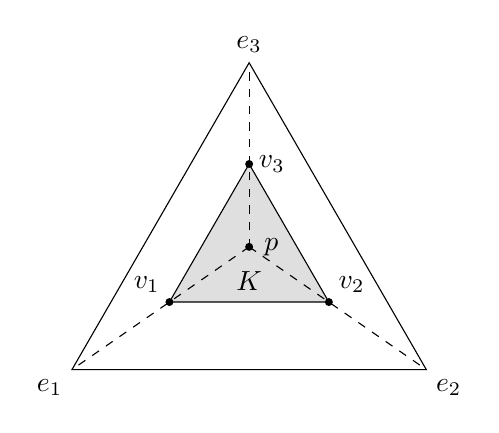
\begin{tikzpicture}[scale=0.9]
  \coordinate (E1) at (0,0); \coordinate (E2) at (5,0); \coordinate (E3) at (2.5,4.330);
  \coordinate (P) at (2.5,1.732);
  \coordinate (V1) at (1.375,0.953); \coordinate (V2) at (3.625,0.953);
  \coordinate (V3) at (2.5,2.901);
  \draw (E1)--(E2)--(E3)--cycle;
  \fill[gray!25] (V1)--(V2)--(V3)--cycle;
  \draw (V1)--(V2)--(V3)--cycle;
  \draw[dashed] (P)--(E1); \draw[dashed] (P)--(E2); \draw[dashed] (P)--(E3);
  \fill (P) circle (1.6pt) node[right=2pt] {$p$};
  \foreach \v/\l/\pos in {V1/v_1/above left,V2/v_2/above right,V3/v_3/right}
    {\fill (\v) circle (1.6pt) node[\pos] {$\l$};}
  \node[below left] at (E1) {$e_1$}; \node[below right] at (E2) {$e_2$};
  \node[above] at (E3) {$e_3$};
  \node at (2.5,1.25) {$K$};
\end{tikzpicture}
\caption{The contamination model $K$ for $n=3$. Each veto point $v_i$ lies on the segment from
$p$ to the vertex $e_i$.}
\label{fig:contam}
\end{figure}

\begin{definition}[The veto--Brier ranking]\label{def:veto-brier}
At world $i$, compare models on $U$ lexicographically by the pair
\[
  a_i(X)\coloneqq\int_X\bigl[-v_i\cdot h\bigr]^+\,d\mu(h),\qquad b_i(X)\coloneqq-\int_Xh_i\,
  d\mu(h),
\]
lower being better: $X\preceq_iY$ if and only if $(a_i(X),b_i(X))\lexle(a_i(Y),b_i(Y))$, where
$(x_1,x_2)\lexle(y_1,y_2)$ means $x_1<y_1$, or $x_1=y_1$ and $x_2\le y_2$.
\end{definition}

The first level is a \emph{veto}: it charges each accepted gamble $h$ by the amount by which its
expectation under $v_i$ falls below zero. Since $v_i$ moves weight $\varepsilon$ from $p$ towards
world $i$, the veto at $i$ charges acceptances that look wrong from the standpoint of world $i$.
The second level is the score of Section~\ref{sec:setting} with its sign reversed: up to a
constant, it is the payoff-weighted error at world $i$.

\begin{theorem}\label{thm:vb}
Let $n\ge2$, $E=\R^n$, and let $\mu$ be a finite Borel measure on $\R^n$ with the null sets of
Lebesgue measure and $\int\|h\|\,d\mu<\infty$, with models identified up to $\mu$-null sets.
Let $p\in\relint\Delta$ and $0<\varepsilon\le1$, and let $K$, $v_1,\dots,v_n$ and $U=\{h:p\cdot
h>0\}$ be as above. On the models on $U$, the veto--Brier ranking has the following
properties.
\begin{enumerate}[label=(\alph*)]
  \item Each relation $\preceq_i$ is complete and transitive, hence finite-chain consistent. The ranking
  satisfies strict guidance and independence.
  \item Every model on $U$ is weakly dominated by an undominated model. Every undominated model
  is coherent: it is a.e.\ equal to $D_{K^\ast}$ for a credal set $K^\ast$ containing $p$ and at
  least one of the points $v_i$.
  \item $D_K$ is undominated. A model tied at every world with an undominated model is itself
  undominated and coherent. Every incoherent model on $U$ is dominated by an undominated coherent
  model.
  \item $D_K\subseteq U$; and $U$ is open and contains $\partial D_K\setminus\{0\}$, so local
  freedom holds at $D_K$.
\end{enumerate}
Hence the veto--Brier ranking covers $K$ on $U$.
\end{theorem}

The proof is in Appendix~\ref{app:vb}. It follows the classical argument from undominatedness
to coherence, without randomisation: the range of score vectors is convex and compact by Lyapunov's
theorem; Zorn's lemma gives every model an undominated weak dominator; a separation argument
shows that every undominated model minimises a nonnegative weighting of the scores over the
region where its active vetoes vanish; and each such minimiser is a.e.\ an intersection of open
half-spaces, which is coherent.

\smallskip\noindent\textbf{Significance and contrast.} Theorem~\ref{thm:vb} shows that complete,
transitive rankings generated by integrated scores can cover some genuinely imprecise targets.
The veto--Brier world orders do tie distinct models: by Lyapunov's theorem, a non-null $Y
\subseteq U$ has a subset $T$ with $z(T)=z(Y)/2$ in the notation of Appendix~\ref{app:vb}, and
then $T$ and $Y\setminus T$ are tied at every world. They are distinct models: $\sum_ip_i
b_i(Y)=-\int_Yp\cdot h\,d\mu<0$, so $z(Y)\ne0$, and hence $z(T)=z(Y\setminus T)=z(Y)/2\ne0$,
which makes both sets non-null. This is why finite-chain consistency in
Section~\ref{sec:undominated} is the chain condition alone: requiring every cycle to consist of
a.e.-equal models would exclude rankings such as this one. The contrast with
Theorem~\ref{thm:main} is instructive in three respects.
\begin{itemize}
  \item \emph{Ordering structure.} The veto--Brier world orders are total preorders; the ranking of
  Definition~\ref{def:ranking} is in general incomplete and intransitive
  (Example~\ref{ex:intransitive}).
  \item \emph{Reach.} The veto--Brier ranking covers its target on a one-sided domain, and its
  undominated models form a proper subfamily of the coherent models on $U$: by (b) and
  Lemma~\ref{lem:identify}(a), the coherent model $U=D_{\{p\}}$ itself is dominated. Precise
  targets ($\varepsilon=0$) cannot be covered on any one-sided domain by any ranking
  (Proposition~\ref{prop:onesided}(c)). On the same domain $U$, the ranking of
  Definition~\ref{def:ranking} also covers $K$, and with it every full-dimensional credal set $\tilde K$ (one with nonempty
  interior relative to $\aff\Delta$) with $p\in\relint\tilde K$ (Corollary~\ref{cor:domains}(d) and
  Proposition~\ref{prop:onesided}(a),(b)); each veto--Brier ranking is built for one target.
  On $E$, the ranking of Definition~\ref{def:ranking} covers every credal set and makes every
  coherent model undominated.
  \item \emph{Dependence on the target.} The veto points $v_i$ are built from $K$, so the
  veto--Brier ranking encodes its target, just as the ranking of Definition~\ref{def:ranking}
  encodes the coherent class through its test. Neither is offered as an independent justification of coherence.
\end{itemize}

\section{Discussion}\label{sec:discussion}

\subsection{What is established}

Under (M1) and (M2), every incoherent model has a coherent repair that improves uniformly at
every state, by a change that no coherent model could make (Theorem~\ref{thm:repair}). The
ranking built from this distinction satisfies the requirements that coverage places on each
world's comparisons (strict guidance, independence and finite-chain consistency), and two
properties that coverage does not require, disjoint additivity and the absence of ties between
distinct models (Proposition~\ref{prop:structure}); it is the largest relation that accepts only strict
improvements between distinct models and accepts changes available to some coherent model only
as guidance (Proposition~\ref{prop:maximal}). Its undominated models are exactly the coherent
models, every model is weakly dominated by an undominated coherent one, every incoherent model is
uniformly dominated by an undominated coherent one, and it covers every credal set
(Theorem~\ref{thm:main}). On a domain closed under coherent hulls, the same holds for the
coherent models on that domain, and the ranking covers exactly those credal sets $K$ with
$D_K\subseteq U$ a.e.\ and local freedom at $D_K$ (Corollary~\ref{cor:domains}(d)).

Two features of the result deserve emphasis. First, the maximality characterisation does not
replace the repair theorem. Under the instance $\mu\{P_S=0\}=0$ of (M2), property (3) of
Proposition~\ref{prop:maximal} alone protects coherent models (Section~\ref{sec:third}), but it says nothing about whether incoherent models are dominated.
That this restricted ranking still gives every incoherent model a coherent dominator is the
substantive achievement, and it rests entirely on Theorem~\ref{thm:repair}. Second, the result
represents coherence exactly, but it does not derive it. The test ``no coherent model could
make this change'' refers to the coherent class. So the theorem shows that the conditions of
Section~\ref{sec:undominated} can all be met, with undominatedness singling out exactly the
coherent models; it does not show that accuracy comparisons justified independently of coherence force it.

A companion paper \cite{KCMcompanion} treats arbitrary models and rankings. It first derives
the dominance property from conditions that can be checked independently, by a
Knaster--Kuratowski--Mazurkiewicz argument on finite sets of worlds that needs only closed sets
of guaranteed comparisons, together with a compactness step. It then records what follows from
that property. Finally, it reduces the construction of rankings to the existence of specific
improvements, of the kind that Theorem~\ref{thm:repair} supplies; the ranking of
Definition~\ref{def:ranking} is an instance of that construction: its two conditions on
guidance are Proposition~\ref{prop:structure}(b) (guided changes improve the score) and
Lemma~\ref{lem:guidedeverywhere} with Proposition~\ref{prop:protect} (guidance protects coherent
models), and the improvements it asks for are supplied by Theorem~\ref{thm:repair}. Here those
improvements, and
with them the dominance property, are proved directly, and the proofs are self-contained.

\subsection{The third condition of Proposition~\ref{prop:maximal}}\label{sec:third}

Property (3) of Proposition~\ref{prop:maximal} restricts individual comparisons at individual
worlds: whenever some coherent model could make a change, the comparison is accepted at $\omega$
only if it is guided by $\omega$. A weaker, global requirement is protection: every coherent
model is undominated under this ranking. Weaker still is coherent admissibility in the sense of
\cite{KCMcompanion}, a condition on a family of rankings: every coherent model is undominated
under at least one ranking in the family, not necessarily under every one. For the one-member
family consisting of this ranking, coherent admissibility is protection. Under the instance
$\mu\{P_S=0\}=0$ of (M2), property (3) implies protection: if (3) holds at every world and $Y$
weakly dominates a coherent model $C$, then the change from $C$ to $Y$, which $C$ itself could
make, is guided by every world, so $Y=C$ a.e.\ by Lemma~\ref{lem:guidedeverywhere} and the proof
of Proposition~\ref{prop:protect}. But (3) is stronger. It constrains comparisons at a single
world, including comparisons with a coherent model that fall short of weak dominance (in
Example~\ref{ex:intransitive}, $X\preceq_1C$ fails although the change raises the score at
world~$1$), and comparisons between incoherent models. It is not needed for coverage: the
veto--Brier ranking of Section~\ref{sec:vb} covers its target, yet the coherent model
$U=D_{\{p\}}$ is dominated there, which (3) would forbid. Its independent justification remains
open.

\subsection{Scope}

\emph{Gambles.} The set of worlds is arbitrary, but the gambles must form a separable,
norm-closed space of bounded functions containing $\one$, or a gamble bounded below by a
positive constant (Remark~\ref{rem:orderunit}). Separability is used for metrizability of the
state space, for the countable set of worlds in Lemma~\ref{lem:states}(f), for Bochner
integrability of the identity map, on which the score and the minimax lemma rest, and for the
existence of measures satisfying (M1)--(M3) in Lemma~\ref{lem:measure}. Some condition like
the second, a gamble bounded below by a positive constant, is needed: at a world where every gamble pays $0$, no comparison is strict, so every
model is undominated.

\emph{Null sets and the measure.} Models are classes modulo $\mu$, and which models are
incoherent depends on $\mu$. Measures satisfying (M1)--(M3) can be mutually singular. Suppose
that $\dim E\ge2$, fix a world $\omega_0$, and let $E_0\coloneqq\{g\in E:g(\omega_0)=0\}$. Take a
countable dense $D_0\subseteq E_0$ and $x_0\in E_0\setminus(D_0-D_0)$, which exists because
$D_0-D_0$ is countable. The measures $\mu,\mu'$ of Lemma~\ref{lem:measure} built from $D_0$
and from $D_0+x_0$ are carried by the disjoint unions of lines $L\coloneqq D_0+\R\one$ and
$L'\coloneqq(D_0+x_0)+\R\one$. For any credal set $Q$, $D_Q\setminus L'$ is coherent for $\mu$
(it equals $D_Q$ $\mu$-a.e.) but is $\mu'$-null, hence incoherent for $\mu'$, because every
coherent model contains the nonempty open set $D_S$, which has positive $\mu'$-measure.

\emph{Full support and null boundaries.} Condition (M3) is used only to tell distinct credal
sets apart (Lemma~\ref{lem:identify}(a)) and for the local freedom results of
Appendix~\ref{app:onesided}. Condition (M2) has three roles. It makes the optimal weighted
choice in the minimax lemma an ordinary acceptance set; it places every consistent model inside
its coherent hull, which gives the test of Lemma~\ref{lem:test} for whether a coherent model could
make a change; and it makes coherent sets of desirable gambles coincide with the coherent models
modulo $\mu$ (Section~\ref{sec:setting}). Protection uses only its instance $\mu\{P_S=0\}=0$,
which is essential (Example~\ref{ex:PS}).

\emph{The score.} The results hold for integrated payoff under every $\mu$ satisfying (M1) and
(M2). A positive reweighting $w\cdot\mu$ with $\int w(1+\|h\|)\,d\mu<\infty$ again satisfies
(M1)--(M3) whenever $\mu$ does, so it needs no separate treatment. Multiplying the score at each
world by a positive constant leaves the ranking unchanged, since only signs of score differences
enter. We make no claim about other scores.

\subsection{Open questions}

\begin{itemize}
  \item Nonseparable spaces, such as the space of all bounded gambles on an infinite set.
  \item Spaces without a gamble bounded below by a positive constant, such as $c_0$. There the
  uniform margin of Theorem~\ref{thm:repair} is impossible, since every element of $c_0$ has
  infimum at most $0$.
  \item Domains not closed under coherent hulls, already for finitely many worlds.
  \item Other scores: for which accuracy measures do comparable repair theorems hold?
  \item The third condition: can property (3) of Proposition~\ref{prop:maximal} be weakened, for
  instance to protection together with other independently motivated conditions, while a single
  ranking still covers every coherent target? If a family of rankings may share the work,
  coherent admissibility in the sense of \cite{KCMcompanion} is the relevant weakening.
  \item Independent justification: is there an accuracy-based argument for the restriction on
  score comparisons that does not presuppose the coherent class?
\end{itemize}

\appendix

\section{Proofs for Section~\ref{sec:setting}}\label{app:setting}

\begin{proof}[Proof of Lemma~\ref{lem:states}]
(a) For $q\in S$ and $h\in E$, $-\|h\|\one\le h\le\|h\|\one$ gives $|q(h)|\le\|h\|$, with
equality at $h=\one$. So $S$ lies in the dual unit ball; it is weak-$\ast$ closed, since
positivity and normalisation are pointwise conditions; so it is weak-$\ast$ compact by the
Banach--Alaoglu theorem. It is metrizable: let $(h_n)_{n\ge1}$ be dense in the unit ball of $E$ and
put $d(q,r)\coloneqq\sum_{n\ge1}2^{-n}|q(h_n)-r(h_n)|$ for $q,r\in S$. Since $|q(h_n)|\le1$, the
series converges uniformly, so $d$ is weak-$\ast$ continuous on $S\times S$; and $d(q,r)=0$ forces
$q=r$ on a dense subset of the unit ball, hence on $E$ by continuity. So the identity map from $S$
with the weak-$\ast$ topology to $S$ with the metric $d$ is a continuous bijection from a compact
space onto a Hausdorff space, hence a homeomorphism. Convexity is clear.

(b) $\delta_\omega\in S$ gives $P_S(h)\le\inf_\Omega h$. Conversely $h-(\inf_\Omega h)\one\ge0$,
so $q(h)\ge\inf_\Omega h$ for all $q\in S$. Apply this to $-h$ for the second claim.

(c) Each $q$ has norm $1$, so $|P_Q(h)-P_Q(h')|\le\|h-h'\|$. A minimum of linear functions is
concave and positively homogeneous, and $q(\one)=1$ gives the translation rule. So $D_Q$ is an
open convex cone, and $\cl D_Q\subseteq\{P_Q\ge0\}$; if $P_Q(h)=0$, then $h\notin D_Q$ while
$h+t\one\in D_Q$ for $t>0$; hence $\partial D_Q=\cl D_Q\setminus D_Q=\{P_Q=0\}$. $D_S\subseteq
D_Q$ since $P_Q\ge P_S$. If $\sup_\Omega h\le0$, then $q(h)\le0$ for all $q$ by (b). The set
$\conv(Q_1\cup Q_2)$ is the image of $Q_1\times Q_2\times[0,1]$ under the continuous map
$(q_1,q_2,\lambda)\mapsto(1-\lambda)q_1+\lambda q_2$, hence weak-$\ast$ compact and convex, and a
linear function has the same minimum over $Q_1\cup Q_2$ as over this set.

(d) The set is the continuous image of $Q\times S$, so it is compact, and it is convex. The
minimum over $\{(1-\tau)q+\tau s\}$ is the sum of $(1-\tau)P_Q$ and $\tau P_S$.

(e) If $Q_2\subseteq Q_1$, then $P_{Q_2}\ge P_{Q_1}$, so $D_{Q_1}\subseteq D_{Q_2}$. Conversely,
suppose $k\in Q_2\setminus Q_1$. The weak-$\ast$ continuous linear functionals on $E^\ast$ are
the evaluations at elements of $E$, so strict separation of $k$ from the compact convex set
$Q_1$ gives $g\in E$ and $c\in\R$ with $q(g)>c>k(g)$ for all $q\in Q_1$. Put $h\coloneqq
g-c\one$. Then $P_{Q_1}(h)>0$, because the minimum is attained, and $k(h)<0$; so $h\in D_{Q_1}
\setminus D_{Q_2}$.

(f) Let $(h_j)$ be dense in $E$. For all $j,l$ choose $\omega_{j,l}$ and $\omega'_{j,l}$ with
$h_j(\omega_{j,l})<\inf_\Omega h_j+1/l$ and $h_j(\omega'_{j,l})>\sup_\Omega h_j-1/l$, and let
$\Omega_0$ be the set of all these worlds. If $\|h-h_j\|<\eta$, then $\inf_{\Omega_0}h\le
\inf_{\Omega_0}h_j+\eta\le\inf_\Omega h_j+\eta\le\inf_\Omega h+2\eta$, and similarly for
suprema.
\end{proof}

\begin{proof}[Proof of Lemma~\ref{lem:measure}]
Fix $\omega_0\in\Omega$ and put $E_0\coloneqq\{g\in E:g(\omega_0)=0\}$, a separable closed
subspace. Let $(g_k)$ be dense in $E_0$ and $w_k>0$ with $\sum_kw_k=1$ and $\sum_kw_k\|g_k\|<
\infty$, and put $\nu\coloneqq\sum_kw_k\delta_{g_k}$, a Borel probability measure on $E_0$ with
full support and $\int\|g\|\,d\nu<\infty$. Let $\lambda$ be the standard normal distribution on
$\R$, and let $\mu$ be the image of $\nu\otimes\lambda$ under $\Phi(g,t)\coloneqq g+t\one$. The
map $\Phi:E_0\times\R\to E$ is a linear homeomorphism, with inverse $h\mapsto(h-h(\omega_0)
\one,h(\omega_0))$, and the Borel $\sigma$-algebra of $E_0\times\R$ is the product
$\sigma$-algebra, since both factors are separable metric spaces. So $\mu$ is a Borel
probability measure on $E$. (M1): $\int\|h\|\,d\mu\le\int\|g\|\,d\nu+\int|t|\,d\lambda<\infty$.
(M3): a nonempty open $W\subseteq E$ has $\Phi^{-1}(W)\supseteq V\times I$ for nonempty open
$V,I$, so $\mu(W)\ge\nu(V)\lambda(I)>0$. (M2): $P_Q(g+t\one)=P_Q(g)+t$, so $\Phi^{-1}\{P_Q=0\}
=\{(g,t):t=-P_Q(g)\}$, and by Fubini's theorem $\mu\{P_Q=0\}=\int\lambda\{-P_Q(g)\}\,d\nu(g)=0$.

If $E=\R^n$ and $\mu$ has the null sets of Lebesgue measure, then (M3) holds because open sets
have positive Lebesgue measure. For (M2), write $h=y+t\one$ with $y\perp\one$, a linear change
of coordinates. The closed set $\{P_Q=0\}$ meets each line $y+\R\one$ in exactly one point, by
the translation rule, so it is Lebesgue-null by Fubini's theorem, and hence $\mu$-null.
\end{proof}

\begin{proof}[Proof of Lemma~\ref{lem:identify}]
(a) The set $O\cap\{P_Q<0\}$ is open and null, hence empty by (M3). If $h\in O$, then
$h-\eta\one\in O$ for some $\eta>0$, so $P_Q(h)-\eta\ge0$ and $h\in D_Q$. If $D_{Q_1}=D_{Q_2}$
a.e., applying this with $O=D_{Q_1}$ and $O=D_{Q_2}$ gives $D_{Q_1}=D_{Q_2}$, and
Lemma~\ref{lem:states}(e) gives $Q_1=Q_2$.

(b) Steps 1--4 do not use (M2). \emph{Step 1.} $D$ contains $D_S=\{\inf_\Omega h>0\}$, which is open and contains $\one$. So
$\inter D$ is a nonempty open convex cone not containing $0$, and $D\subseteq\cl\inter D$, since
a convex set with nonempty interior lies in the closure of its interior.
\emph{Step 2.} Let $\psi\in E^\ast$ be nonzero and nonnegative on $D$. For $h\ge0$ and $t>0$,
$h+t\one\in D_S\subseteq D$, so $\psi(h)\ge-t\psi(\one)$; hence $\psi$ is positive. Then
$|\psi(h)|\le\|h\|\psi(\one)$, so $\psi(\one)>0$ and $\psi/\psi(\one)\in K_D$. So the nonzero
functionals nonnegative on $D$ are the positive multiples of members of $K_D$.
\emph{Step 3.} By the Hahn--Banach theorem there is $\varphi\in E^\ast$ with $\varphi>0$ on the
open convex set $\inter D$, which misses $0$. By Step 1, $\varphi\ge0$ on $D$, so $K_D\ne
\emptyset$ by Step 2. $K_D$ is weak-$\ast$ closed and convex, so it is a credal set.
\emph{Step 4.} $\cl D$ is a closed convex cone, so by the bipolar theorem and Step 2, $\cl D=
C_{K_D}$. Hence $D\subseteq C_{K_D}$, and $D_{K_D}$, being open and contained in $\cl D$, is
contained in $\inter\cl D=\inter D\subseteq D$; here $\inter\cl D=\inter D$ because $D$ is convex
with nonempty interior.
\emph{Step 5.} Assume (M2). Then $D\setminus D_{K_D}\subseteq C_{K_D}\setminus D_{K_D}=\{P_{K_D}=0\}$, which is
null by (M2). So $D$ differs from the open set $D_{K_D}$ by a subset of a null set, and $D=
D_{K_D}$ a.e.

(c) $D_Q\cup\{h\ge0:h\ne0\}$ is a convex cone, since $P_Q(h+g)\ge P_Q(h)+P_Q(g)\ge
P_Q(h)$ for $g\ge0$; it excludes $0$, and it contains every nonzero $h\ge0$. Its difference from
$D_Q$ lies in $\{P_Q=0\}$, because $h\ge0$ gives $P_Q(h)\ge0$; so it is null by (M2).
\end{proof}

\section{Examples delimiting the main results}\label{app:examples}

Both examples use $\Omega=(0,1]$ and $E\coloneqq\{a+b\,\omega:a,b\in\R\}$, a two-dimensional
subspace of $\ell^\infty(\Omega)$ containing $\one$, which we identify with $\R^2$ through the
coefficients $(a,b)$. Positivity applied to $\omega$ and $\one-\omega$ shows that the states are
$q_s(a+b\,\omega)\coloneqq a+bs$ with $s\in[0,1]$; the state $q_0$ is not an evaluation. So
$P_S(a+b\,\omega)=\min(a,a+b)$ and $D_S=\{a>0,\ a+b>0\}$.

\begin{example}\label{ex:nonuniform}
This example shows that dominance need not be uniform. Let $\mu$ be the standard Gaussian distribution of the
coefficients. Since $\one$ corresponds to $(1,0)$, the argument of Lemma~\ref{lem:measure} for
$\R^n$ applies verbatim, and $\mu$ satisfies (M1)--(M3). Let $V$ be an open ball in coefficient
space. By Lyapunov's theorem in the form proved by Lindenstrauss \cite{Lyapunov,Lindenstrauss},
the range of the non-atomic vector measure $Y\mapsto m(Y)$ on the measurable subsets of $V$
is $\{\int_Vf\,h\,d\mu:0\le f\le1\}$. Hence the set
\[
  R\coloneqq\{m(A_1)-m(V\setminus A_1):A_1\subseteq V\}=\Bigl\{\int_V(2f-1)\,h\,d\mu:f
  \text{ measurable},\ 0\le f\le1\Bigr\}
\]
is compact, convex and symmetric about $0$. Its support function in a direction $\lambda\ne0$
is $\int_V|\lambda\cdot h|\,d\mu>0$, since $V$ is non-null and $\{\lambda\cdot h=0\}$ is null;
being continuous on the unit circle, it is at least some $c>0$ there. A compact convex set whose
support function is at least $c$ in every unit direction contains every point $y$ with $|y|<c$
(otherwise a separating direction $\lambda$ would give $c\le\lambda\cdot y<c$). Let $A_0$ be an
open ball inside $D_S$ and disjoint from $V$, small enough that $|m(A_0)|<c/2$, and let $0<\beta
<c/2$. Then $(0,\beta)-m(A_0)\in R$, so some $A_1\subseteq V$ has $m(A_1)-m(V\setminus A_1)=
(0,\beta)-m(A_0)$. Put $Y\coloneqq A_0\cup A_1$ and $X\coloneqq V\setminus A_1$. The change from
$X$ to $Y$ adds $A_0\cup A_1$ and removes $V\setminus A_1$, and $m(Y)-m(X)$ is the gamble
$\beta\,\omega$. No coherent model could make this change: either $V\setminus A_1$ is
inconsistent, or $\hull(V\setminus A_1)\supseteq D_S\supseteq A_0$, which is non-null
(Lemma~\ref{lem:test}). By Proposition~\ref{prop:strict}, $Y$ strictly dominates $X$, with score
gain $\beta\,\omega$ at the world $\omega$; its infimum over $\Omega$ is $0$, so the dominance is
not uniform.
\end{example}

\begin{example}\label{ex:PS}
This example shows that the null boundary $\{P_S=0\}$ in (M2) is essential for protection. Let
$\mu$ be the sum of the standard Gaussian distribution of the coefficients and the distribution
of $(0,\theta)$ with $\theta$ exponentially distributed. Then $\mu$ is finite and has full support, and (M1) holds. But the ray $R\coloneqq
\{a=0,\ b>0\}$ has $\mu(R)=1$ and lies in $\{P_S=0\}$, so (M2) fails. Let $Q\coloneqq\{q_s:0\le
s\le\frac12\}$; then $C\coloneqq D_Q=\{a>0,\ a+b/2>0\}$ is coherent and disjoint from $R$. Every
$h=b\,\omega\in R$ is positive at every world, so the change from $C$ to $C\cup R$, which adds
$R$, is guided by every world, and $C\cup R\preceq_\omega C$ at every $\omega$. The reverse
change removes gambles that pay off at $\omega$, so it is not guided, and its score difference
$-m_\omega(R)$ is negative. Hence $C\cup R$ strictly dominates the coherent model $C$.
\end{example}

\begin{remark}\label{rem:orderunit}
The constant gamble $\one$ can be replaced by any gamble bounded below by a positive constant.
Suppose that $E$ contains some $e$ with $\inf_\Omega e>0$, but not
necessarily $\one$. Define states by positivity and $q(e)=1$. The map $h\mapsto h/e$ is a
linear bijection of $E$ onto $\tilde E\coloneqq\{h/e:h\in E\}$, bounded with bounded inverse
since $\|h/e\|\le\|h\|/\inf_\Omega e$ and $\|h\|\le\|e\|\,\|h/e\|$; so $\tilde E$ is a closed
separable subspace of $\ell^\infty(\Omega)$ containing $\one$. The map preserves the sign of
every gamble at every world, and hence guidance. Setting $\tilde q(h/e)\coloneqq q(h)$ maps
states to states with $P_{\tilde Q}(h/e)=P_Q(h)$, so it preserves the sets $D_Q$, the
conditions (M1)--(M3) for the image measure, the coherent models and the test of
Lemma~\ref{lem:test}. Finally $m_\omega(X)=e(\omega)\,\tilde m_\omega(\tilde X)$ with
$e(\omega)>0$, where $\tilde X$ is the image of $X$ and $\tilde m$ the score for the image
measure; so the ranking is preserved, and all results transfer, with margins multiplied by at
least $\inf_\Omega e$.
\end{remark}

\section{One-sided domains}\label{app:onesided}

\begin{definition}[One-sided domains and the common annihilator]\label{def:one-sided}
A domain $V$ is \emph{one-sided} if no nonempty open set $O$ has both $O\subseteq V$ a.e.\ and
$-O\subseteq V$ a.e. Under (M3), each $D_{K'}$ is one-sided: if $O$ and $-O$ lie in $D_{K'}$
a.e., Lemma~\ref{lem:identify}(a) puts $O$ inside $D_{K'}\cap(-D_{K'})$, which is empty. For a
credal set $K$ let $K_\perp\coloneqq\{h\in E:k(h)=0\text{ for all }k\in K\}$.
\end{definition}

\begin{proposition}\label{prop:onesided}
Assume (M1)--(M3). Let $K'$ and $K$ be credal sets and $U\coloneqq D_{K'}$.
\begin{enumerate}[label=(\alph*)]
  \item The ranking on $U$ covers $K$ if and only if $K'\subseteq K$ and every $k\in K'$
  satisfies $k(h)>0$ for all $h\in C_K\setminus\{0\}$. No ranking on $U$ covers $K$ unless
  this condition holds.
  \item If $E=\R^n$, the condition in (a) holds if and only if $K$ has nonempty interior
  relative to the affine hull of $\Delta$ and $K'\subseteq\relint K$.
  \item If $K_\perp\ne\{0\}$, local freedom at $D_K$ fails on every one-sided domain, so no
  ranking on a one-sided domain covers $K$. If $E$ is infinite-dimensional, this applies to
  every $K$ that is the convex hull of finitely many states, in particular to every precise
  $K=\{p\}$.
\end{enumerate}
\end{proposition}

\begin{proof}
By Lemma~\ref{lem:states}(c), $\partial D_K\setminus\{0\}=\{h\ne0:P_K(h)=0\}\subseteq C_K
\setminus\{0\}$.

(a) By Corollary~\ref{cor:domains}(d) it suffices to show that the condition is equivalent to
``$D_K\subseteq U$ a.e.\ and local freedom at $D_K$''. By Lemmas~\ref{lem:identify}(a)
and~\ref{lem:states}(e), $D_K\subseteq U$ a.e.\ if and only if $K'\subseteq K$. If the
condition holds, every $h\in\partial D_K\setminus\{0\}$ has $k(h)>0$ for all $k\in K'$, so
$P_{K'}(h)>0$ (the minimum is attained), and the open set $U$ contains $\partial D_K\setminus
\{0\}$. Conversely, let $O\supseteq\partial D_K\setminus\{0\}$ be open with $O\subseteq U$ a.e.;
then $O\subseteq U$ by Lemma~\ref{lem:identify}(a). If $k\in K'$ and $h\in C_K\setminus\{0\}$ had
$k(h)=0$, then $0\le P_K(h)\le k(h)=0$ since $k\in K$, so $h\in\partial D_K\setminus\{0\}
\subseteq U$, contradicting $P_{K'}(h)\le k(h)=0$.

(b) Here $S=\Delta$. Every affine function on $\aff\Delta$ has the form $m\mapsto m\cdot h$,
since $a\cdot m+c=(a+c\one)\cdot m$ there. Suppose $K$ has nonempty relative interior and $k\in
\relint K$, and let $h\in C_K\setminus\{0\}$ with $k\cdot h=0$. If $m\mapsto m\cdot h$ were
constant on $\aff\Delta$, it would be $0$ and $h=0$; otherwise some $d$ with $\one\cdot d=0$ has
$d\cdot h\ne0$, and one of $(k\pm td)\cdot h=\pm t\,d\cdot h$ is negative for small $t>0$, while
$k\pm td\in K$. This is a contradiction. Conversely, if $K$ has empty relative interior, its
linear span has dimension less than $n$, so some $h\ne0$ has $m\cdot h=0$ on $K$; and if $k\in
K'$ lies on the relative boundary of $K$, a supporting hyperplane to $K$ at $k$ in $\aff\Delta$
\cite[Thm.~11.6]{Rockafellar} gives a non-constant affine function, hence some $h\ne0$, with
$m\cdot h\ge0=k\cdot h$ on $K$. Either way the condition fails.

(c) Let $0\ne h\in K_\perp$. Then $P_K(\pm h)=0$, so $\pm h\in\partial D_K\setminus\{0\}$. If an
open $O\supseteq\partial D_K\setminus\{0\}$ lay in a domain $V$ a.e., a ball $W$ about $h$ with
$W\cup(-W)\subseteq O$ would have $W\subseteq V$ and $-W\subseteq V$ a.e., so $V$ would not be
one-sided. If $K=\conv\{k_1,\dots,k_m\}$, then $K_\perp=\bigcap_i\ker k_i$ has codimension at most
$m$, so it is nonzero when $E$ is infinite-dimensional.
\end{proof}

\section{Proof of Theorem~\ref{thm:vb}}\label{app:vb}

Throughout, $\varphi_i(h)\coloneqq[-v_i\cdot h]^+$, so that $a_i(X)=\int_X\varphi_i\,d\mu$ and
$b_i(X)=-m_i(X)$; models are models on $U$; and $|h|_\infty\coloneqq\max_j|h_j|$. Since $v_i\in
\Delta$, $0\le\varphi_i\le|h|_\infty$, so all scores are finite.

\emph{Step 1: the sign condition.} If $h\in U$ and $h_i\ge0$, then $v_i\cdot h=(1-\varepsilon)
p\cdot h+\varepsilon h_i\ge0$, so $\varphi_i(h)=0$. Also $-h_i<0$ on $\{h_i>0\}$ and $-h_i>0$ on
$\{h_i<0\}$.

\emph{Step 2: part (a).} $\lexle$ is a total order on $\R^2$, so each $\preceq_i$ is complete
and transitive, and a.e.-equal models are tied. The differences $a_i(X)-a_i(Y)=\int_{X\setminus
Y}\varphi_i\,d\mu-\int_{Y\setminus X}\varphi_i\,d\mu$ and $b_i(X)-b_i(Y)$ depend only on the
change from $Y$ to $X$, and $x\lexle y$ if and only if $0\lexle y-x$; this is independence. If
the change from $Y$ to $X$ is guided by $i$ and non-null, then $\varphi_i=0$ a.e.\ on $X\setminus
Y$ by Step 1, so $a_i(X)-a_i(Y)=-\int_{Y\setminus X}\varphi_i\le0$, and $b_i(X)-b_i(Y)=
-\int_{X\setminus Y}h_i+\int_{Y\setminus X}h_i<0$. So $X\prec_iY$: strict guidance.

\emph{Step 3: the range.} Put
\[
  z(X)\coloneqq\bigl(a_1(X),\dots,a_n(X),b_1(X),\dots,b_n(X)\bigr)=\int_X\psi\,d\mu,\qquad
  \psi\coloneqq(\varphi_1,\dots,\varphi_n,-h_1,\dots,-h_n),
\]
where $\psi$ is integrable on $U$. Since $\mu$
has Lebesgue's null sets, it has no atoms, so by Lyapunov's theorem
\cite{Lyapunov,Lindenstrauss} the range $Z\coloneqq\{z(X)\}$ is a compact convex subset of
$\R^{2n}$, and $0=z(\emptyset)\in Z$. For $y,y'\in\R^{2n}$ write $y\trianglelefteq y'$ if
$(y_{a_i},y_{b_i})\lexle(y'_{a_i},y'_{b_i})$ for every $i$, where $y_{a_i},y_{b_i}$ are the
coordinates in the positions of $a_i,b_i$. This is a partial order. A model $Y$ weakly dominates
$X$ if and only if $z(Y)\trianglelefteq z(X)$; it dominates $X$ if and only if, in addition,
$z(Y)\ne z(X)$; and $X,Y$ are tied at every world if and only if $z(X)=z(Y)$. So whether a model
is dominated depends only on its score vector.

\emph{Step 4: undominated weak dominators.} Fix a model $X_0$ and put $D\coloneqq\{y\in Z:y
\trianglelefteq z(X_0)\}$. We show that every chain in $D$ has a lower bound in $D$; the empty
chain has $z(X_0)$. Let $\mathcal K\subseteq D$ be a nonempty chain. For $\gamma\in\mathcal
K$ let $T_\gamma\coloneqq\{\gamma'\in\mathcal K:\gamma'\trianglelefteq\gamma\}$. Finitely many
sets $T_\gamma$ have a common element (the least of their indices), so the closed sets $\cl
T_\gamma$ have the finite intersection property, and by compactness some $y^\infty\in Z$ lies in
all of them. Fix $\gamma$ and $i$. Every $\gamma'\in T_{\gamma''}$ has $\gamma'_{a_i}\le
\gamma''_{a_i}$, so $y^\infty_{a_i}\le\gamma''_{a_i}$ for all $\gamma''\in\mathcal K$. If
$y^\infty_{a_i}<\gamma_{a_i}$, then $(y^\infty_{a_i},y^\infty_{b_i})\lexlt(\gamma_{a_i},
\gamma_{b_i})$. Otherwise $\gamma_{a_i}=y^\infty_{a_i}\le\gamma'_{a_i}\le\gamma_{a_i}$ for
$\gamma'\in T_\gamma$, so $a_i$ is constant on $T_\gamma$, the lexicographic order gives
$\gamma'_{b_i}\le\gamma_{b_i}$ there, and $y^\infty_{b_i}\le\gamma_{b_i}$ by closure. Hence
$y^\infty\trianglelefteq\gamma$ for all $\gamma$, and $y^\infty\in D$ is a lower bound of
$\mathcal K$. By Zorn's lemma, $D$ has a minimal element $y^\ast$; a model $X^\ast$ with
$z(X^\ast)=y^\ast$ weakly dominates $X_0$, and a dominator of $X^\ast$ would contradict
minimality. This proves the first claim of (b).

\emph{Step 5: separation.} Let $X^\ast$ be undominated and $W_0\coloneqq\{\omega:a_\omega(X^\ast)
=0\}$. If $W_0=\emptyset$, then $\emptyset$ strictly dominates $X^\ast$; so $W_0\ne\emptyset$.
Since $\varphi_\omega\ge0$, $X^\ast\subseteq N(W_0)\coloneqq U\cap\bigcap_{\omega\in W_0}
\{\varphi_\omega=0\}$ a.e. Let $Z'\coloneqq\{y\in Z:y_{a_\omega}=0\text{ for }\omega\in W_0\}$,
a convex set containing $z(X)$ for every model $X\subseteq N(W_0)$, and $y^\ast\coloneqq
z(X^\ast)$. Let $\mathrm{pr}$ project $\R^{2n}$ onto the coordinates $y_{b_\omega}$ ($\omega\in
W_0$) and $y_{a_\omega},y_{b_\omega}$ ($\omega\notin W_0$), and let $P$ be the nonempty open
convex cone of vectors $d$ with $d_{b_\omega}<0$ for $\omega\in W_0$ and $d_{a_\omega}<0$ for
$\omega\notin W_0$. If $\mathrm{pr}(y-y^\ast)\in P$ for some $y\in Z'$, the model realising $y$
would be strictly better than $X^\ast$ at every world. So the convex set $\mathrm{pr}(Z'-y^\ast)$,
which contains $0$, is disjoint from $P$. By the separation theorem
\cite[Thm.~11.3]{Rockafellar} there is a linear functional $\Lambda\ne0$ with $\sup_P\Lambda
\le\inf_{\mathrm{pr}(Z'-y^\ast)}\Lambda$; since $0$ lies in $\mathrm{pr}(Z'-y^\ast)$ and in
$\cl P$, both sides are $0$, so $\Lambda\le0$ on $\cl P$ and $\Lambda\ge0$ on
$\mathrm{pr}(Z'-y^\ast)$. Write $\Lambda(d)=
\sum_{\omega\in W_0}\beta_\omega d_{b_\omega}+\sum_{\omega\notin W_0}(\alpha_\omega d_{a_\omega}+
\gamma_\omega d_{b_\omega})$. Testing on $\cl P$ gives $\beta,\alpha\ge0$ and $\gamma=0$. Extend
$\beta$ by $0$ outside $W_0$. Then $X^\ast$ minimises $J\coloneqq\sum_{\omega\in W_0}\beta_\omega
b_\omega+\sum_{\omega\notin W_0}\alpha_\omega a_\omega$ over the models $X\subseteq N(W_0)$. If
$\beta=0$, then $\alpha\ne0$, $J\ge0$ on $Z'$ and $J(0)=0$, so $J(y^\ast)=0$, forcing
$a_\omega(X^\ast)=0$ for some $\omega\notin W_0$ with $\alpha_\omega>0$, contrary to the
definition of $W_0$. So $\beta\ne0$, and $\one\cdot\beta>0$.

\emph{Step 6: uniqueness.} For $X\subseteq N(W_0)$, $J(X)=\int_Xg\,d\mu$ with
\[
  g(h)\coloneqq\sum_{\omega\notin W_0}\alpha_\omega[-v_\omega\cdot h]^+-\beta\cdot h .
\]
For $t\ge0$, $[-v_\omega\cdot(h+t\one)]^+\le[-v_\omega\cdot h]^+$ and $\beta\cdot(h+t\one)=
\beta\cdot h+t\,\one\cdot\beta$, so $t\mapsto g(h+t\one)$ is strictly decreasing. The closed set
$\{g=0\}$ therefore meets each line $h+\R\one$ at most once, and it is null by the Fubini
argument of Lemma~\ref{lem:measure}. Since $\int_Xg\,d\mu\ge\int_{N(W_0)\cap\{g<0\}}g\,d\mu$, with
equality if and only if $X=N(W_0)\cap\{g<0\}$ a.e., we get $X^\ast=N(W_0)\cap\{g<0\}$ a.e.

\emph{Step 7: coherence.} For a nonempty compact $T\subseteq\Delta$, a linear function has the
same minimum over $T$ as over its compact convex hull, so $D_T=D_{\conv T}$ and $D_{T_1}\cap
D_{T_2}=D_{T_1\cup T_2}$. Each hyperplane $\{v_\omega\cdot h=0\}$ is null, so $N(W_0)=
D_{\{p\}\cup\{v_\omega:\omega\in W_0\}}$ a.e. Since $[-v\cdot h]^+=\max_{0\le t\le1}(-t\,v\cdot
h)$ and $\alpha\ge0$,
\[
  g(h)=\max_{w\in W}(-w\cdot h),\qquad W\coloneqq\Bigl\{\beta+\sum_{\omega\notin W_0}
  \alpha_\omega t_\omega v_\omega:t\in[0,1]^{\Omega\setminus W_0}\Bigr\}.
\]
$W$ is compact, and each $w\in W$ is nonnegative with $\one\cdot w\ge\one\cdot\beta>0$. So
$\{g<0\}=D_{\hat W}$, where $\hat W\coloneqq\{w/(\one\cdot w):w\in W\}\subseteq\Delta$ is
compact. Hence $X^\ast=D_{K^\ast}$ a.e., where $K^\ast\coloneqq\conv
\bigl(\{p\}\cup\{v_\omega:\omega\in W_0\}\cup\hat W\bigr)$ is a credal set containing $p$ and
$v_\omega$ for $\omega\in W_0\ne\emptyset$. This completes (b).

\emph{Step 8: part (c).} For $h\in D_K$, $v_i\cdot h>0$ since $v_i\in K$, so $a_i(D_K)=0$. Let
$Y$ weakly dominate $D_K$. Then $a_i(Y)=0$ for every $i$, so $Y\subseteq N(\Omega)=D_{\{p,v_1,
\dots,v_n\}}=D_K$ a.e., using $p\in K=\conv\{v_1,\dots,v_n\}$. With the first levels tied,
$b_i(Y)\le b_i(D_K)$ for every $i$, and so
\[
  0\ge\sum_ip_i\bigl(b_i(Y)-b_i(D_K)\bigr)=\int_{D_K\setminus Y}p\cdot h\,d\mu ,
\]
whereas $p\cdot h>0$ on $D_K$. Hence $D_K\setminus Y$ is null and $Y=D_K$ a.e.; so $D_K$ is
undominated. If $Y$ is tied at every world with an undominated $X$, then $z(Y)=z(X)$, so $Y$ is
undominated by Step 3, and coherent by Step 7. Finally, let $X$ be incoherent, and let $Y$ be an
undominated weak dominator (Step 4), coherent by Step 7. If $Y$ did not dominate $X$, the two
would be tied at every world, so $X$ would be undominated and hence coherent. So $Y$ dominates
$X$.

\emph{Step 9: part (d).} The map $m\mapsto(1-\varepsilon)p+\varepsilon m$ is an affine bijection
of $\aff\Delta$ that fixes $p$ and maps $\Delta$ onto $K$; so $K$ has nonempty relative
interior and $p\in\relint K$. Since $p\in K$, $D_K\subseteq U$. Let $h\in\partial D_K\setminus
\{0\}$. Then $h\in C_K\setminus\{0\}$, and the argument in the proof of
Proposition~\ref{prop:onesided}(b) gives $p\cdot h>0$, that is, $h\in U$. As $U$ is open, local
freedom holds with neighbourhood $U$.
\qed

\begin{thebibliography}{99}

\bibitem{BergerDas}
D.~Berger and N.~Das.
\newblock Accuracy and credal imprecision.
\newblock \emph{No\^us}, 54:666--703, 2020.

\bibitem{deFinetti}
B.~de~Finetti.
\newblock \emph{Theory of Probability}, volume~1.
\newblock Wiley, 1974.

\bibitem{DiestelUhl}
J.~Diestel and J.~J. Uhl.
\newblock \emph{Vector Measures}.
\newblock American Mathematical Society, 1977.

\bibitem{Joyce}
J.~M. Joyce.
\newblock A nonpragmatic vindication of probabilism.
\newblock \emph{Philosophy of Science}, 65:575--603, 1998.

\bibitem{Konek}
J.~Konek.
\newblock Epistemic conservativity and imprecise credence.
\newblock \emph{Philosophy and Phenomenological Research}, forthcoming.
% year, volume, pages to be supplied by the author

\bibitem{KCMcompanion}
J.~Konek and C.~Campbell-Moore.
\newblock Coherence and dominance under general rankings.
\newblock Manuscript, 2026.

\bibitem{Lindenstrauss}
J.~Lindenstrauss.
\newblock A short proof of {L}iapounoff's convexity theorem.
\newblock \emph{Journal of Mathematics and Mechanics}, 15:971--972, 1966.

\bibitem{Lyapunov}
A.~Lyapunov.
\newblock Sur les fonctions-vecteurs compl\`etement additives.
\newblock \emph{Izvestiya Akademii Nauk SSSR, Seriya Matematicheskaya}, 4:465--478, 1940.

\bibitem{MayoWilsonWheeler}
C.~Mayo-Wilson and G.~Wheeler.
\newblock Scoring imprecise credences: a mildly immodest proposal.
\newblock \emph{Philosophy and Phenomenological Research}, 93:55--78, 2016.

\bibitem{Pettigrew}
R.~Pettigrew.
\newblock \emph{Accuracy and the Laws of Credence}.
\newblock Oxford University Press, 2016.

\bibitem{Predd}
J.~B. Predd, R.~Seiringer, E.~H. Lieb, D.~N. Osherson, H.~V. Poor, and S.~R. Kulkarni.
\newblock Probabilistic coherence and proper scoring rules.
\newblock \emph{IEEE Transactions on Information Theory}, 55:4786--4792, 2009.

\bibitem{Quaeghebeur}
E.~Quaeghebeur.
\newblock Desirability.
\newblock In T.~Augustin, F.~P.~A. Coolen, G.~de~Cooman, and M.~C.~M. Troffaes, editors,
\emph{Introduction to Imprecise Probabilities}, pages 1--27. Wiley, 2014.

\bibitem{Rockafellar}
R.~T. Rockafellar.
\newblock \emph{Convex Analysis}.
\newblock Princeton University Press, 1970.

\bibitem{Schoenfield}
M.~Schoenfield.
\newblock The accuracy and rationality of imprecise credences.
\newblock \emph{No\^us}, 51:667--685, 2017.

\bibitem{SSK}
T.~Seidenfeld, M.~J. Schervish, and J.~B. Kadane.
\newblock Forecasting with imprecise probabilities.
\newblock \emph{International Journal of Approximate Reasoning}, 53:1248--1261, 2012.

\bibitem{Sion}
M.~Sion.
\newblock On general minimax theorems.
\newblock \emph{Pacific Journal of Mathematics}, 8:171--176, 1958.

\bibitem{Walley}
P.~Walley.
\newblock \emph{Statistical Reasoning with Imprecise Probabilities}.
\newblock Chapman and Hall, 1991.

\end{thebibliography}

\end{document}
